\documentclass {article}
\usepackage[utf8]{inputenc}
\usepackage{fontenc}
\usepackage[english]{babel}
\usepackage[%hypertex,
                 unicode=true,
                 plainpages = false, 
                 pdfpagelabels, 
                 bookmarks=true,
                 bookmarksnumbered=true,
                 bookmarksopen=true,
                 breaklinks=true,
                 backref=false,
                 colorlinks=true,
                 linkcolor = blue,		% Use "blue" if you want to highlight them
                 urlcolor  = blue,
                 citecolor = red,
                 anchorcolor = green,
                 hyperindex = true,
                 linktocpage = true,
                 hyperfigures
]{hyperref}
\usepackage{graphicx}
\usepackage{float}
\usepackage{fancyhdr}
\usepackage{listingsutf8}
\usepackage{xcolor}
\graphicspath{{figures/PNG/}{figures/PDF/}{figures/}}
\usepackage{amsfonts}
\usepackage{amsmath}
\usepackage{amssymb}	
\usepackage{wrapfig}
\usepackage{enumitem}
\usepackage{subfigure}
\usepackage{amssymb}
\usepackage{amsmath}
\usepackage [a4paper, top=2.5cm, bottom=2cm, left=1.5cm, right=1.5cm] {geometry}
\pagestyle{fancy}

% cambiato bottom da 1.8 + logo

\makeatletter
\@addtoreset{section}{part}
\makeatother
\rhead{\large Schr\"{o}dinger equation and Jacobi's method}

\lhead{\large Project 2}
\lfoot{D. Brugnara, M. Cammilli, M. Seclì}
\cfoot{}
\rfoot{\thepage}
\renewcommand{\headrulewidth}{0.7pt}
\renewcommand{\footrulewidth}{0.7pt}

\definecolor{dkgreen}{rgb}{0,0.6,0}
\definecolor{dred}{rgb}{0.545,0,0}
\definecolor{dblue}{rgb}{0,0,0.545}
\definecolor{lgrey}{rgb}{0.9,0.9,0.9}
\definecolor{gray}{rgb}{0.4,0.4,0.4}
\definecolor{darkblue}{rgb}{0.0,0.0,0.6}
\lstdefinelanguage{cpp}{
      backgroundcolor=\color{lgrey},  
      basicstyle=\footnotesize \ttfamily \color{black} \bfseries,   
      breakatwhitespace=false,       
      breaklines=true,               
      captionpos=b,                   
      commentstyle=\color{dkgreen},   
      deletekeywords={...},          
      escapeinside={\%*}{*)},                  
      frame=single,                  
      language=C++,                
      keywordstyle=\color{purple},  
      morekeywords={BRIEFDescriptorConfig,string,TiXmlNode,DetectorDescriptorConfigContainer,istringstream,cerr,exit}, 
      identifierstyle=\color{black},
      stringstyle=\color{blue},      
      numbers=right,                 
      numbersep=5pt,                  
      numberstyle=\tiny\color{black}, 
      rulecolor=\color{black},        
      showspaces=false,               
      showstringspaces=false,        
      showtabs=false,                
      stepnumber=1,                   
      tabsize=5,                     
      title=\lstname,                 
    }

\author{
%\textbf{\normalsize Gruppo A6:}\\
\normalsize Daniele Brugnara \texttt{$<$\href{mailto:daniebru@mail.uio.no}
{daniebru@mail.uio.no}$>$}\\
\normalsize Martina Cammilli \texttt{$<$\href{mailto:marticam@mail.uio.no}
{marticam@mail.uio.no}$>$}\\
\normalsize Matteo Seclì \texttt{$<$\href{mailto:mattes@mail.uio.no}
{mattes@mail.uio.no}$>$}\\
}

\title{\textbf{Schrödinger's equation for two electrons in a three dimensional harmonic oscillator well}}

\begin{document}

\maketitle

\hrule
%\medskip
\begin{center}
	\large\textbf{Abstract}
	\medskip\\
	\begin{minipage}[c][][c]{0.8\textwidth}
		\small{
			The aim of this project is to solve numerically the Schrödinger equation for a three dimensional harmonic potential with one and two electrons. In order to solve this problem, we will rewrite it as an eigenvalue problem to be solved with Jacobi's rotation method; we will then discuss its efficiency and accuracy. As a result, we will obtain -- for $l=0$ -- the radial solutions for one and two electrons and their respective probabilities densities. The latter allow us to make predictions about the electrons position and have an intuitive picture of how electrons interactions affect the solution of the problem.}
	\end{minipage}
\end{center}
\medskip
\hrule

\tableofcontents

\section{Introduction}

\subsection{Single electron}

It is possible to break the usual Schrödinger equation in various decoupled differential equations.

\begin{equation}
i \hbar \frac{\partial}{\partial t} \Psi(\vec{r}, t)= \hat{H} \Psi(\vec{r}, t)
\end{equation}

Using polar coordinates, for a potential that depends only on $r$, the distance from the origin, it is possible to derive a radial equation as follows:

\begin{equation}
-\frac{\hbar}{2m} \left( \frac{1}{r^2}\frac{d}{dr}r^2 \frac{d}{dr}-\frac{l(l+1)}{r^2} \right) R(r)+ \frac{1}{2} m \omega^2 r^2 R(r)=E R(r)
\label{diffeq}
\end{equation}

where we have considered the harmonic potential $V(r)=\frac{1}{2} m \omega^2 r^2$

Setting $l=0$ for simplicity (we're only interested in solutions with no angular momentum), through some algebraic passages and substitutions, we obtain the following differential equation:

\begin{equation}
- \frac{d^2}{d \rho^2} u(\rho) +\rho^2 u(\rho)=\lambda u(\rho) \quad \quad \mbox{where} \quad \lambda=\frac{2 m \alpha^2}{\hbar^2}E \mbox{,} \quad \alpha=\left( \frac{\hbar^2}{mk} \right)^{\frac{1}{4}} \mbox{,} \quad \rho=\frac{1}{\alpha} r \quad \mbox{and} \quad R(r)=\frac{1}{r}u(r)
\end{equation}

Notice that the possible eigenvalues are 3, 7, 11 and so on, because:
\begin{align}
\lambda_n &= \frac{2 m \alpha^2}{\hbar^2}E_n \\
          &= \frac{2 m \alpha^2}{\hbar^2} \frac{1}{2}\hbar \omega (4n+3) \\
          &= \frac{m\omega \alpha^2}{\hbar}(4n + 3) \\
          &= \frac{m \omega}{\hbar}\sqrt{\frac{\hbar^2}{m^2 \omega^2}}(4n+3) \\
          &= 4n + 3
          \label{eq:seria}
\end{align}

Considering the following expression for the second derivative (3 points formula), it is possible to discretize the problem through matrix operations.

\begin{equation}
\frac{d^2}{d \rho^2} u(\rho)=\frac{u(\rho-h)-2 u(\rho)+u(\rho+h)}{h^2} +O(h^2)
\end{equation}

It is also possible to write the differential equation (\ref{diffeq}) as a matrix product and then exploit the Jacobi rotation algorithm to compute the eigenvalues $\lambda$ of the equation and the eigenfunctions that solve it.

\subsection{Two electrons}

Let's introduce the relative coordinates $\vec r=\vec r_2-\vec r_1$ and $\vec R=\frac{\vec r_1 + \vec r_2}{2}$. The Schrodinger equation becomes the following:

\begin{equation}
\left(- \frac{\hbar^2}{n} \frac{d^2}{dr^2}-\frac{\hbar^2}{4n} \frac{d^2}{dR^2}+\frac{1}{4} k r^2+kR^2+ \frac{\beta e^2}{r} \right)u(r, R)=\left(E_1 + E_2 \right) u(R, r)
\end{equation}

With the separation of variables technique, it is possible once again to break down the equation and consider only the relative position for now. With the appropriate substitutions, we obtain the following differential equation:

\begin{equation}
- \frac{d^2}{d \rho^2} u(\rho) +\left(\omega_r^2 \rho^2 +\frac{1}{\rho} \right) u(\rho)=\lambda u(\rho) \quad \quad \mbox{where} \quad \omega_r=\frac{mk}{4 \hbar^2} \alpha^4 \quad \mbox{and} \quad \alpha=\frac{\hbar^2}{m \beta e^2}
\label{chc}
\end{equation}

\section{Jacobi's rotation}

Jacobi' algorithm allows us to diagonalize a symmetric matrix through successive rotations performed by unitary matrices as follows, exploiting the property of the product in equation (\ref{basechange}) of not changing the eigenvalues of matrix $A$.

\begin{equation}
B=R_i^T A R_i \Longrightarrow D=R_n^T\dots R_1^T A R_1 \dots R_n
\label{basechange}
\end{equation}

The unitary matrix is of the form:

\begin{equation}
\begin{pmatrix}
   1 & 0 &  0 & 0 & \cdots & 0  \\
  0 &  \cos(\theta) & 0 & \cdots & -\sin(\theta) & 0  \\
   0 & 0 &  1 & 0 & \cdots & 0 \\   
  \vdots  & \vdots  & & \ddots & & \vdots   \\
   0 &  \sin(\theta) & \cdots  & 0 & \cos(\theta) & 0 \\
   0 &  0 & \cdots & \cdots  & 0 & 1
 \end{pmatrix}
 \quad \quad\mbox{the position of $\cos(\theta)$ is $k$ and $l$}
\end{equation}

It is possible to show that the elements of the rotated matrix are the following:

\begin{align}
b_{i, i}&=a_{i, i} & \mbox{if} \quad i\neq k, l\\
b_{i, k}&=a_{i, k} \cos (\theta) - a_{i, l} \sin(\theta) & \mbox{if} \quad i\neq k, l\\
b_{i, l}&=a_{i, l} \cos (\theta) + a_{i, k} \sin(\theta) & \mbox{if} \quad i\neq k, l\\
b_{k, k}&=a_{k, k} \cos^2 (\theta) -2 a_{k, l} \sin (\theta) \cos (\theta)+ a_{l, l} \sin^2(\theta) &\\
b_{l, l}&=a_{l, l} \cos^2 (\theta) +2 a_{k, l} \sin (\theta) \cos (\theta)+ a_{k, k} \sin^2(\theta) &\\
b_{k, l}&=(a_{k, l}-a_{l, l} )\cos (\theta) \sin(\theta)+ a_{k, l}(\cos^2(\theta)- \sin^2 (\theta)) &
\label{values}
\end{align}

Choosing $k$ and $l$ as the indexes of the highest element every time a rotation is performed, and choosing the correct angle $\theta$ that cancels the $b_{k, l}$ element, we can obtain a matrix that is "more diagonal" for each step. We do not know however how many steps it will take with this algorithm to fully diagonalize the matrix.
Setting $b_{k, l}$ equal to zero we obtain the following condition on the value of $\cos(\theta)$:

\begin{align}
b_{k, l}=0&=(a_{k, l}-a_{l, l} )\cos (\theta) \sin(\theta)+ a_{k, l}(\cos^2(\theta)- \sin^2 (\theta)) &\\
&=\cos^2 (\theta)) +2 \tau \cos(\theta) \sin( \theta)- \sin^2 (\theta)= & \mbox{where} \quad \tau=\frac{a_{k, l}-a_{l, l}}{2 a_{k, l} } \\
& \Longrightarrow \cot (\theta)=-\tau \pm \sqrt{\tau^2+1} &\\
& \Longrightarrow \cos(\theta) =\frac{1}{\sqrt{1+ \cot^{-2}(\theta)}} &
\label{condition}
\end{align}

Let's consider the function that performs the rotation broken down in pieces:
\begin{lstlisting}[language=cpp]
   void rotate ( mat& A, mat& R, int k, int l, int n ) {
    // Compute the values of cos and sin
    double s, c;
    if ( A(k,l) != 0.0 ) {
        double t, tau;
        tau = (A(l,l) - A(k,k))/(2*A(k,l));
        if ( tau > 0 ) {
            t = 1.0/(tau + sqrt(1.0 + tau*tau));
        } else {
            t = -1.0/( -tau + sqrt(1.0 + tau*tau));
        }
        c = 1/sqrt(1+t*t);
        s = c*t;
    } else {
        c = 1.0;
        s = 0.0;
    }   
\end{lstlisting}

This first part first checks whether the chosen element is in fact different from zero. If it is, it proceeds to compute the value of t as required by the previous equation (\ref{condition}), choosing the higher root so that the value of the tangent is the smallest, since it's the inverse. Lastly the required values of sine and cosine are computed.

If however the element was already zero, the values of sine and cosine are defined as respectively 0 and 1, so that the element remains equal to zero (in fact it's easy to check that the rotation matrix is the identity).

The next part of the code creates the new rotated matrix. Note that only the needed elements are changed, avoiding the costly operation of double matrix multiplication.
\begin{lstlisting}[language=cpp]
    // Change the elements that have to be changed
    double a_kk, a_ll, a_ik, a_il, r_ik, r_il;
    a_kk = A(k,k);
    a_ll = A(l,l);
    // Changing the matrix elements with indices k and l
    A(k,k) = c*c*a_kk - 2.0*c*s*A(k,l) + s*s*a_ll;
    A(l,l) = s*s*a_kk + 2.0*c*s*A(k,l) + c*c*a_ll;
    A(k,l) = 0.0;
    A(l,k) = 0.0;
    for ( int i = 0; i < n; i++ ) {
        // Changing the remaining elements
        if ( i != k && i != l ) {
            a_ik = A(i,k);
            a_il = A(i,l);
            A(i,k) = c*a_ik - s*a_il;
            A(k,i) = A(i,k);
            A(i,l) = c*a_il + s*a_ik;
            A(l,i) = A(i,l);
        }
        // Compute the new eigenvectors
        r_ik = R(i,k);
        r_il = R(i,l);
        R(i,k) = c*r_ik - s*r_il;
        R(i,l) = c*r_il + s*r_ik;
    }
\end{lstlisting}

The first step performed is to set equal to zero the elements with indexes ${k, l}$ and ${l, k}$. Then the script proceeds to computing the values of the other matrix elements that have changed according to equations (\ref{values}).

Lastly the matrix product $R''^T=R'^T \times R^T$ is computed, where $R'$ is the matrix product of all the previous rotation matrices, that, once the matrix is diagonalized is composed by all the eigenvectors. However the actual matrix multiplication is not needed since the only elements that change are the following ones:

\begin{equation*}
R''_{i, k}=\cos(\theta) R'_{i, k}-\sin(\theta) R'_{i, l} 
\end{equation*}

\begin{equation*}
R''_{i, l}=\cos(\theta) R'_{i, l}+\sin(\theta) R'_{i, k} 
\end{equation*}

The rest of the script, which we will not show here is composed by a function that finds the higher off-diagonal element and then calls the Jacobi rotation function, checking everything whether the absolute value of the higher off-diagonal element is lower than a precision parameter $\epsilon$ that can be set up by the user.

\subsection{Execution time and precision}
Unfortunately this algorithm doesn't have a fixed number of iterations to diagonalize the matrix, as a consequence, the number of rotations and therefore the time needed for the diagonalization varies upon the matrix itself. In figure (\ref{pff}) we can see the  elapsed time to diagonalize matrices of different dimensions using the Jacobi rotation and the \texttt{eig\_gen} function integrated in the Armadillo library. We notice a clear difference that tells us that the Jacobi rotation is not the best algorithm to diagonalize a already tridiagonal matrix and that much more efficient methods can be implemented.

\begin{figure}[H]
	\centering
	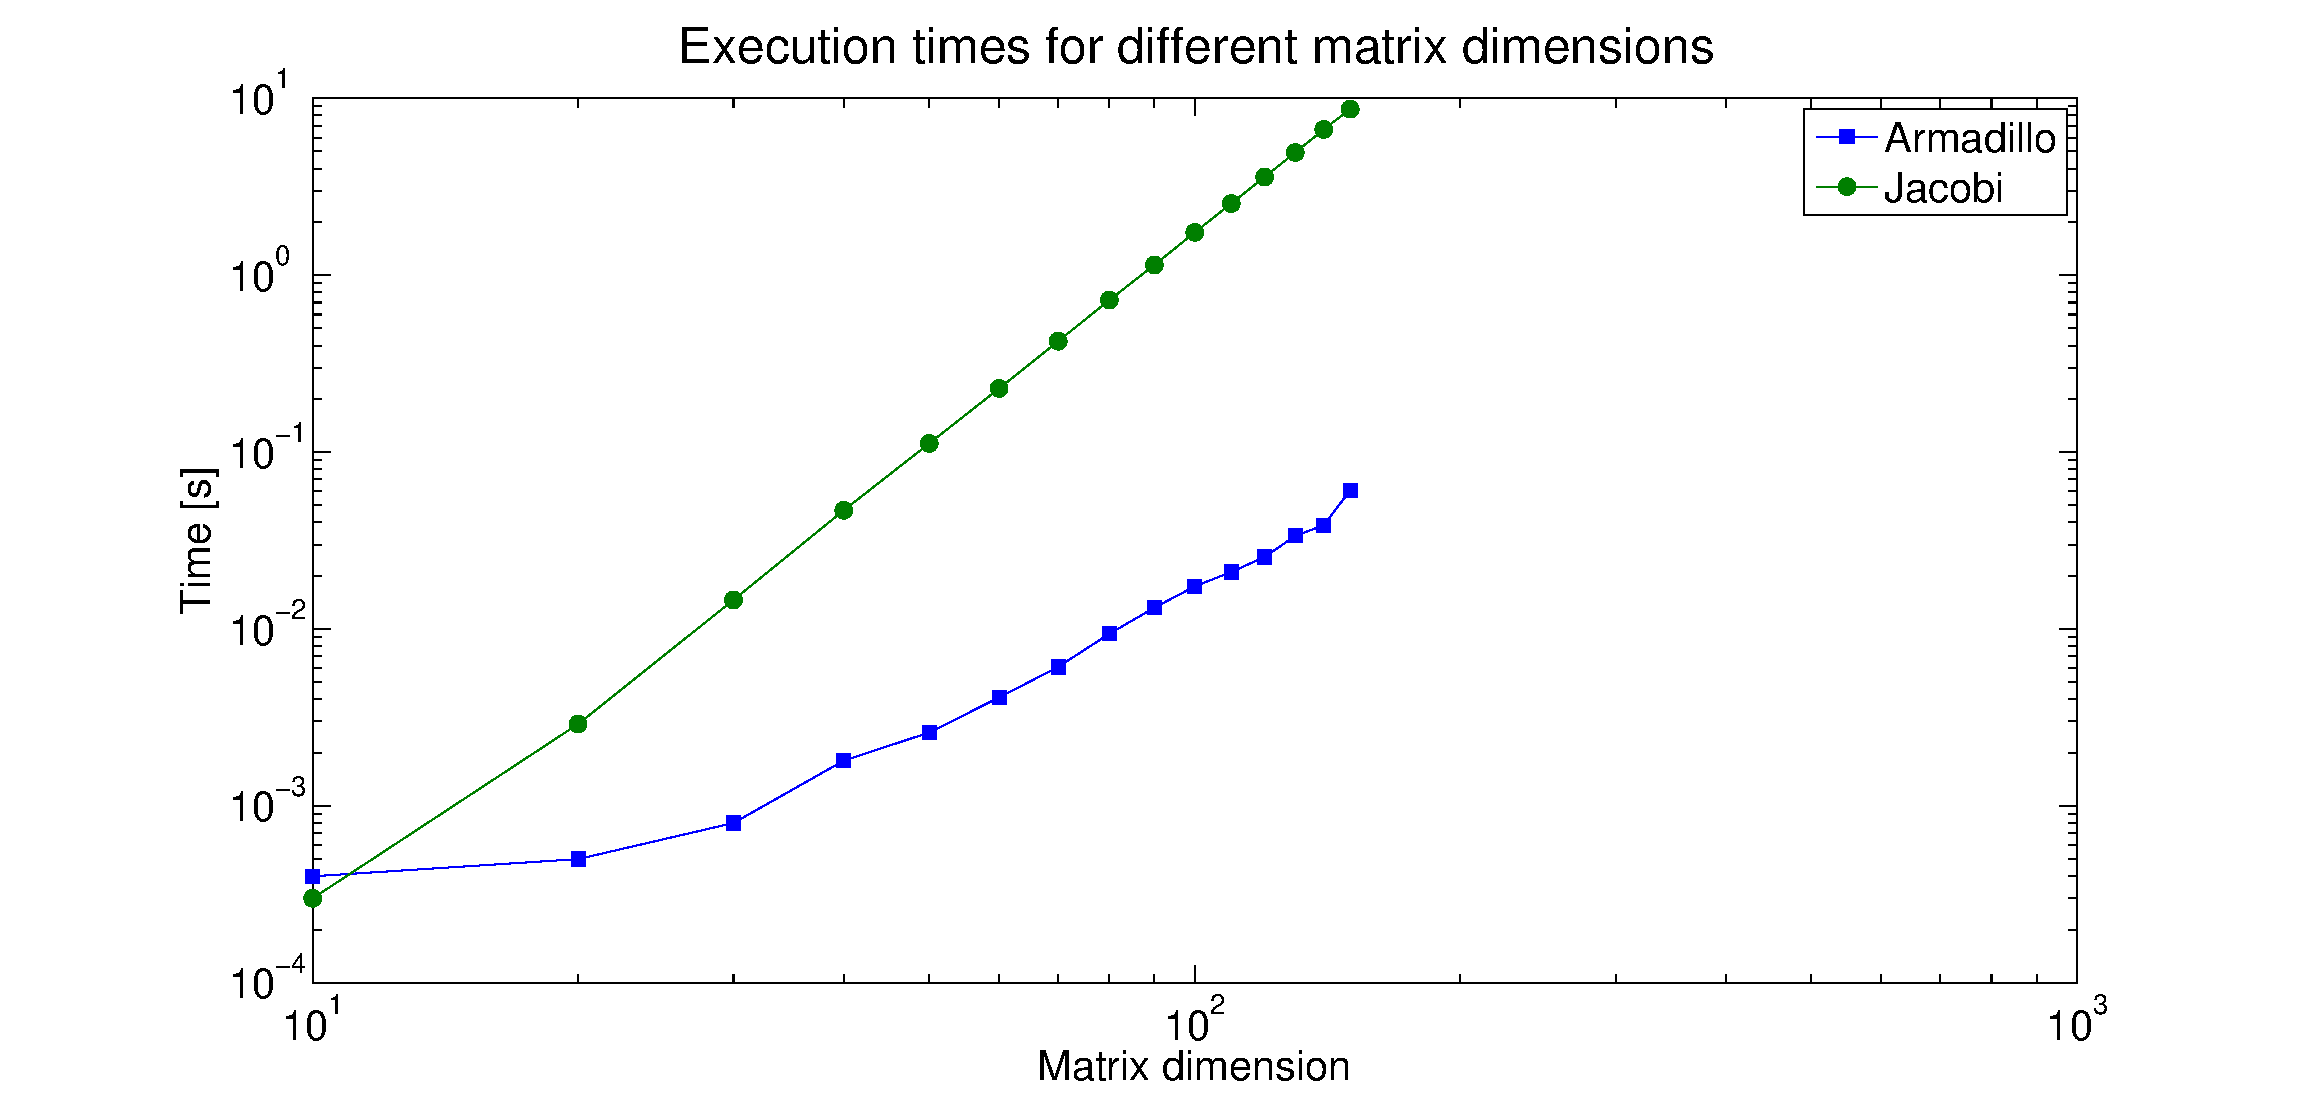
\includegraphics[width=16cm]{times}
	\caption{We notice that Armadillo has a much more fast algorithm to perform the diagonalization of a tridiagonal square matrix. Obviously, both algorithms grow slower at the increasing of the matrix's dimension. The grid is logarithmic.}
	\label{pff}
\end{figure}

In Figure \ref{fig:iterations} we can also see how the number of rotations depends on the dimension of the matrix. A quick fit of the data reveals that such a number is proportional to the square of the matrix dimension ($\simeq n^{2.10}$). This is to be expected since the number of elements in a matrix is indeed the square of its dimension. 

\begin{figure}[H]
	\centering
	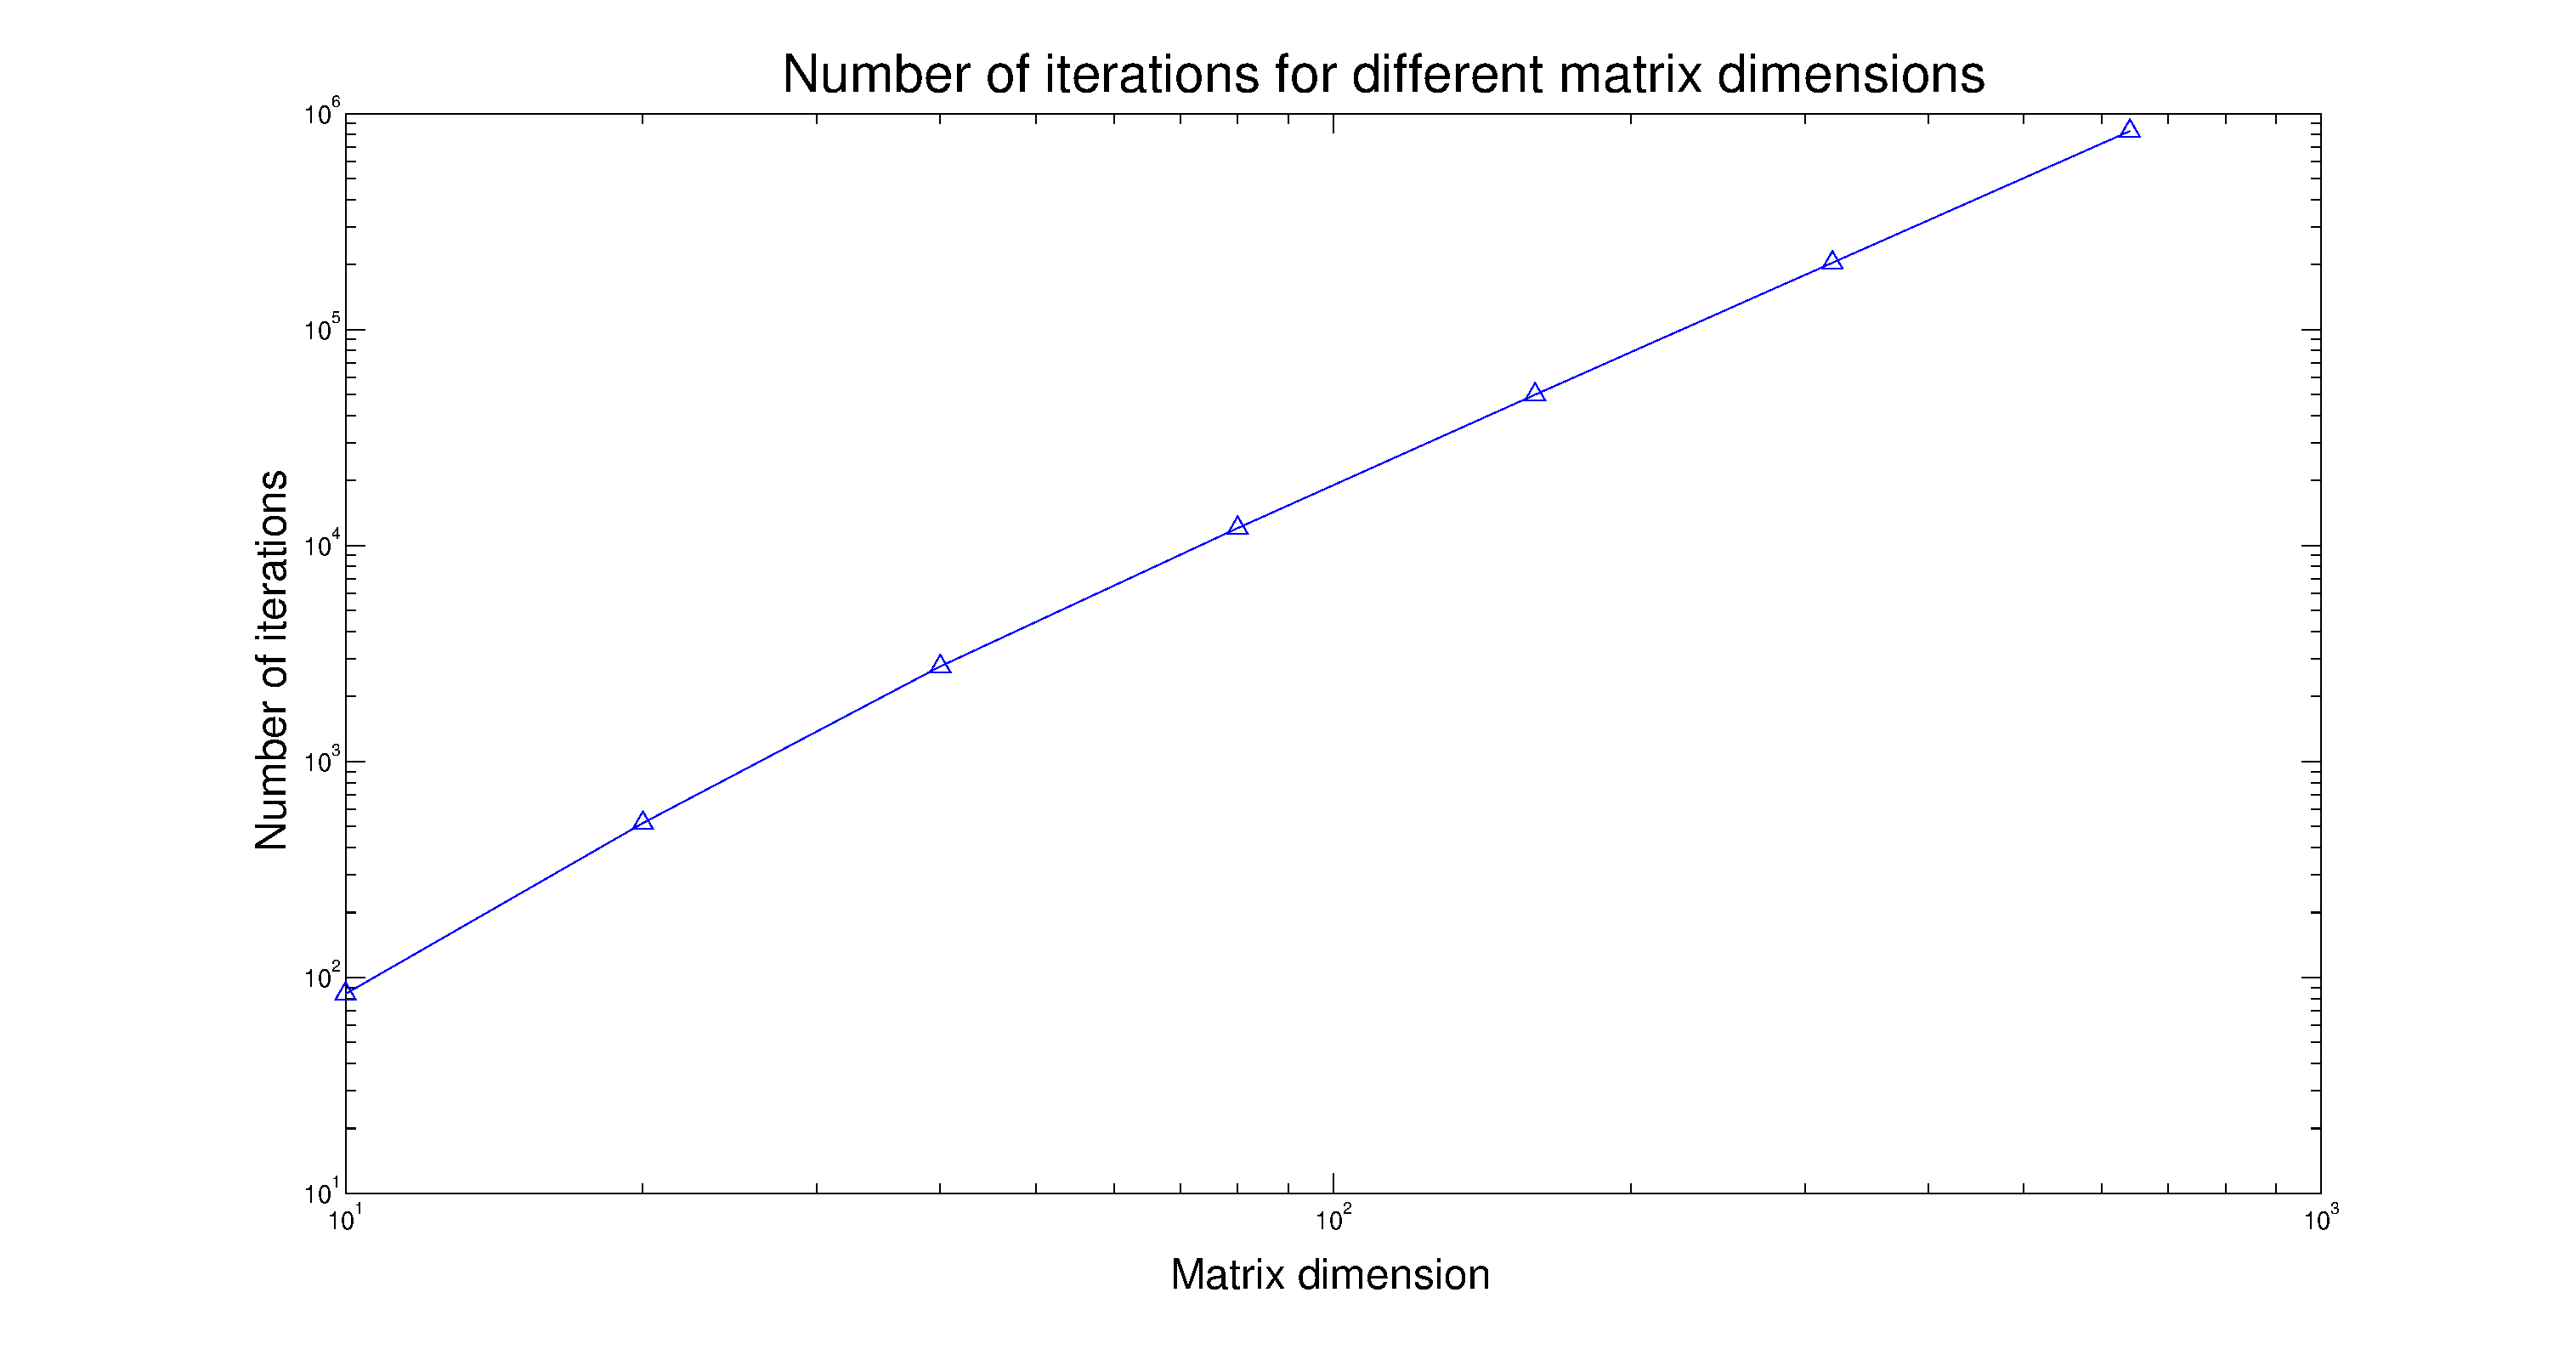
\includegraphics[width=16cm]{casascemo}
	\caption{Number of iterations as a function of the matrix dimension.}
	\label{fig:iterations}
\end{figure}

As expected, the relative error lowers by increasing the dimension of the matrix. It is evident from Figure \ref{fig:errors} that we need approximately $700$ points to reach a precision of order $10^{-4}$. In fact, with less than $\simeq 600$ points the eigenvalues that we obtain with our algorithm have less than four leading digits (compared to the theoretical ones in equation (\ref{eq:seria})).

\begin{figure}[H]
	\centering
	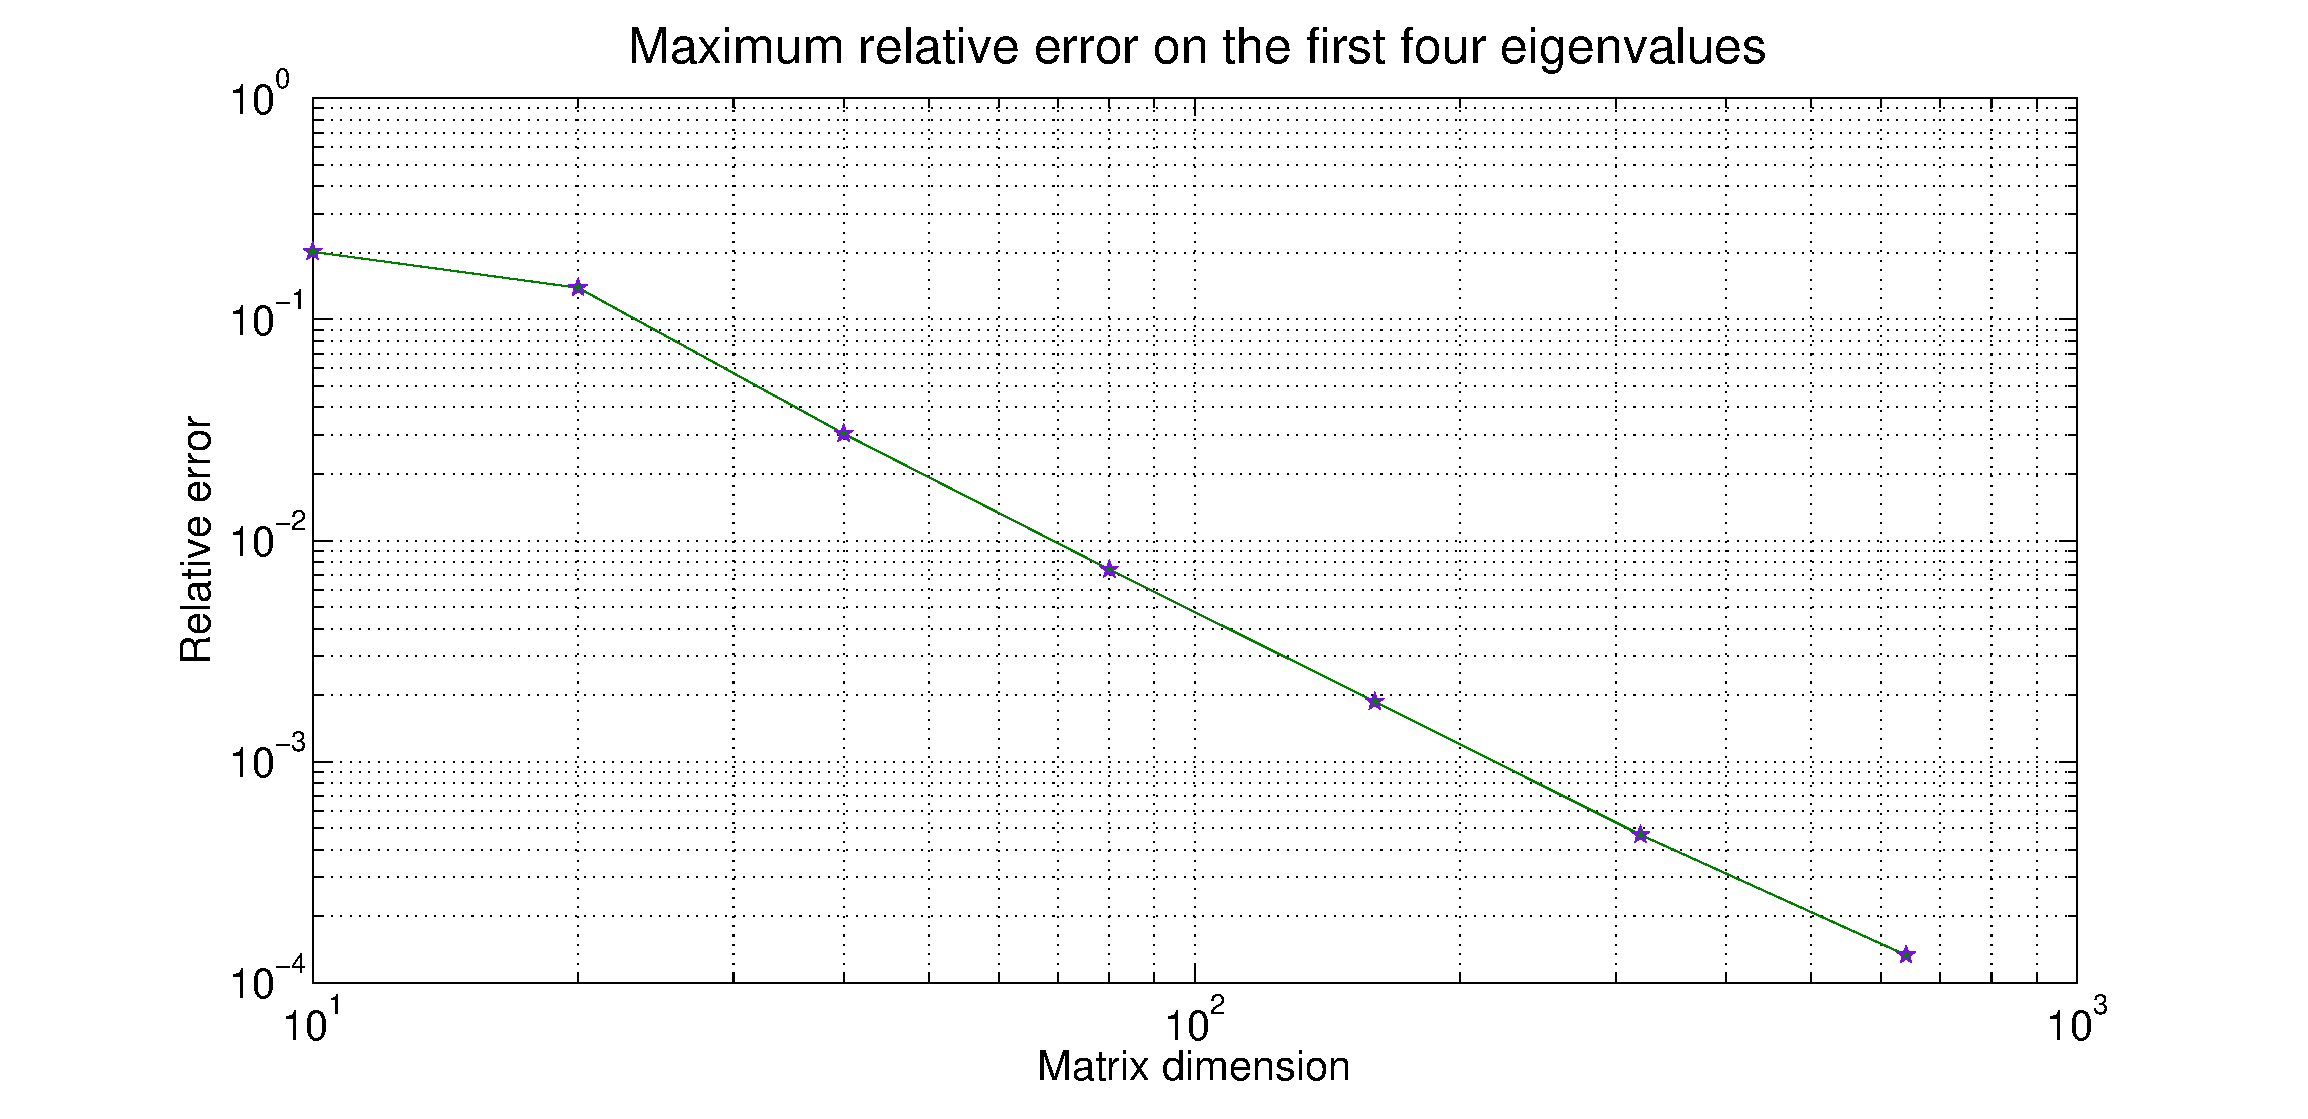
\includegraphics[width=16cm]{errors}
	\caption{Maximum relative error on the first four eigenvalues as a function of the matrix dimension.}
	\label{fig:errors}
\end{figure}

\section{Single electron in an harmonic potential}

Here in Figure \ref{fig:energy_levels_one_electron} we show the energy levels -- that are proportional to $\lambda$ -- for $\rho_{\max}=10$ and $n=500$. As explained before we expect that the eigenvalues go as a straight line, but it's evident that there are fluctuations for the first and the last eigenvalues. This is due to the fact that the theoretical space in which we are working is an Hilbert space with infinite dimension, while here we have a matrix space of dimension $500$. Secondly, we set $\rho_{\max}=10$ instead of the theoretical $\rho_{\max}=\infty$, meaning we did a strong approximation. The ideal thing to do is to set a high $\rho_{max}$, but then the step length on which we discretize our solution is much more high, meaning we have less significant points per unit length. To balance this effect we should also increase the matrix dimension, but a certain point it becomes computationally impossible to diagonalize a huge matrix. So, the solution is a compromise between the matrix dimension and the choice of the point that plays the role of infinity.

\begin{figure}[H]
	\centering
	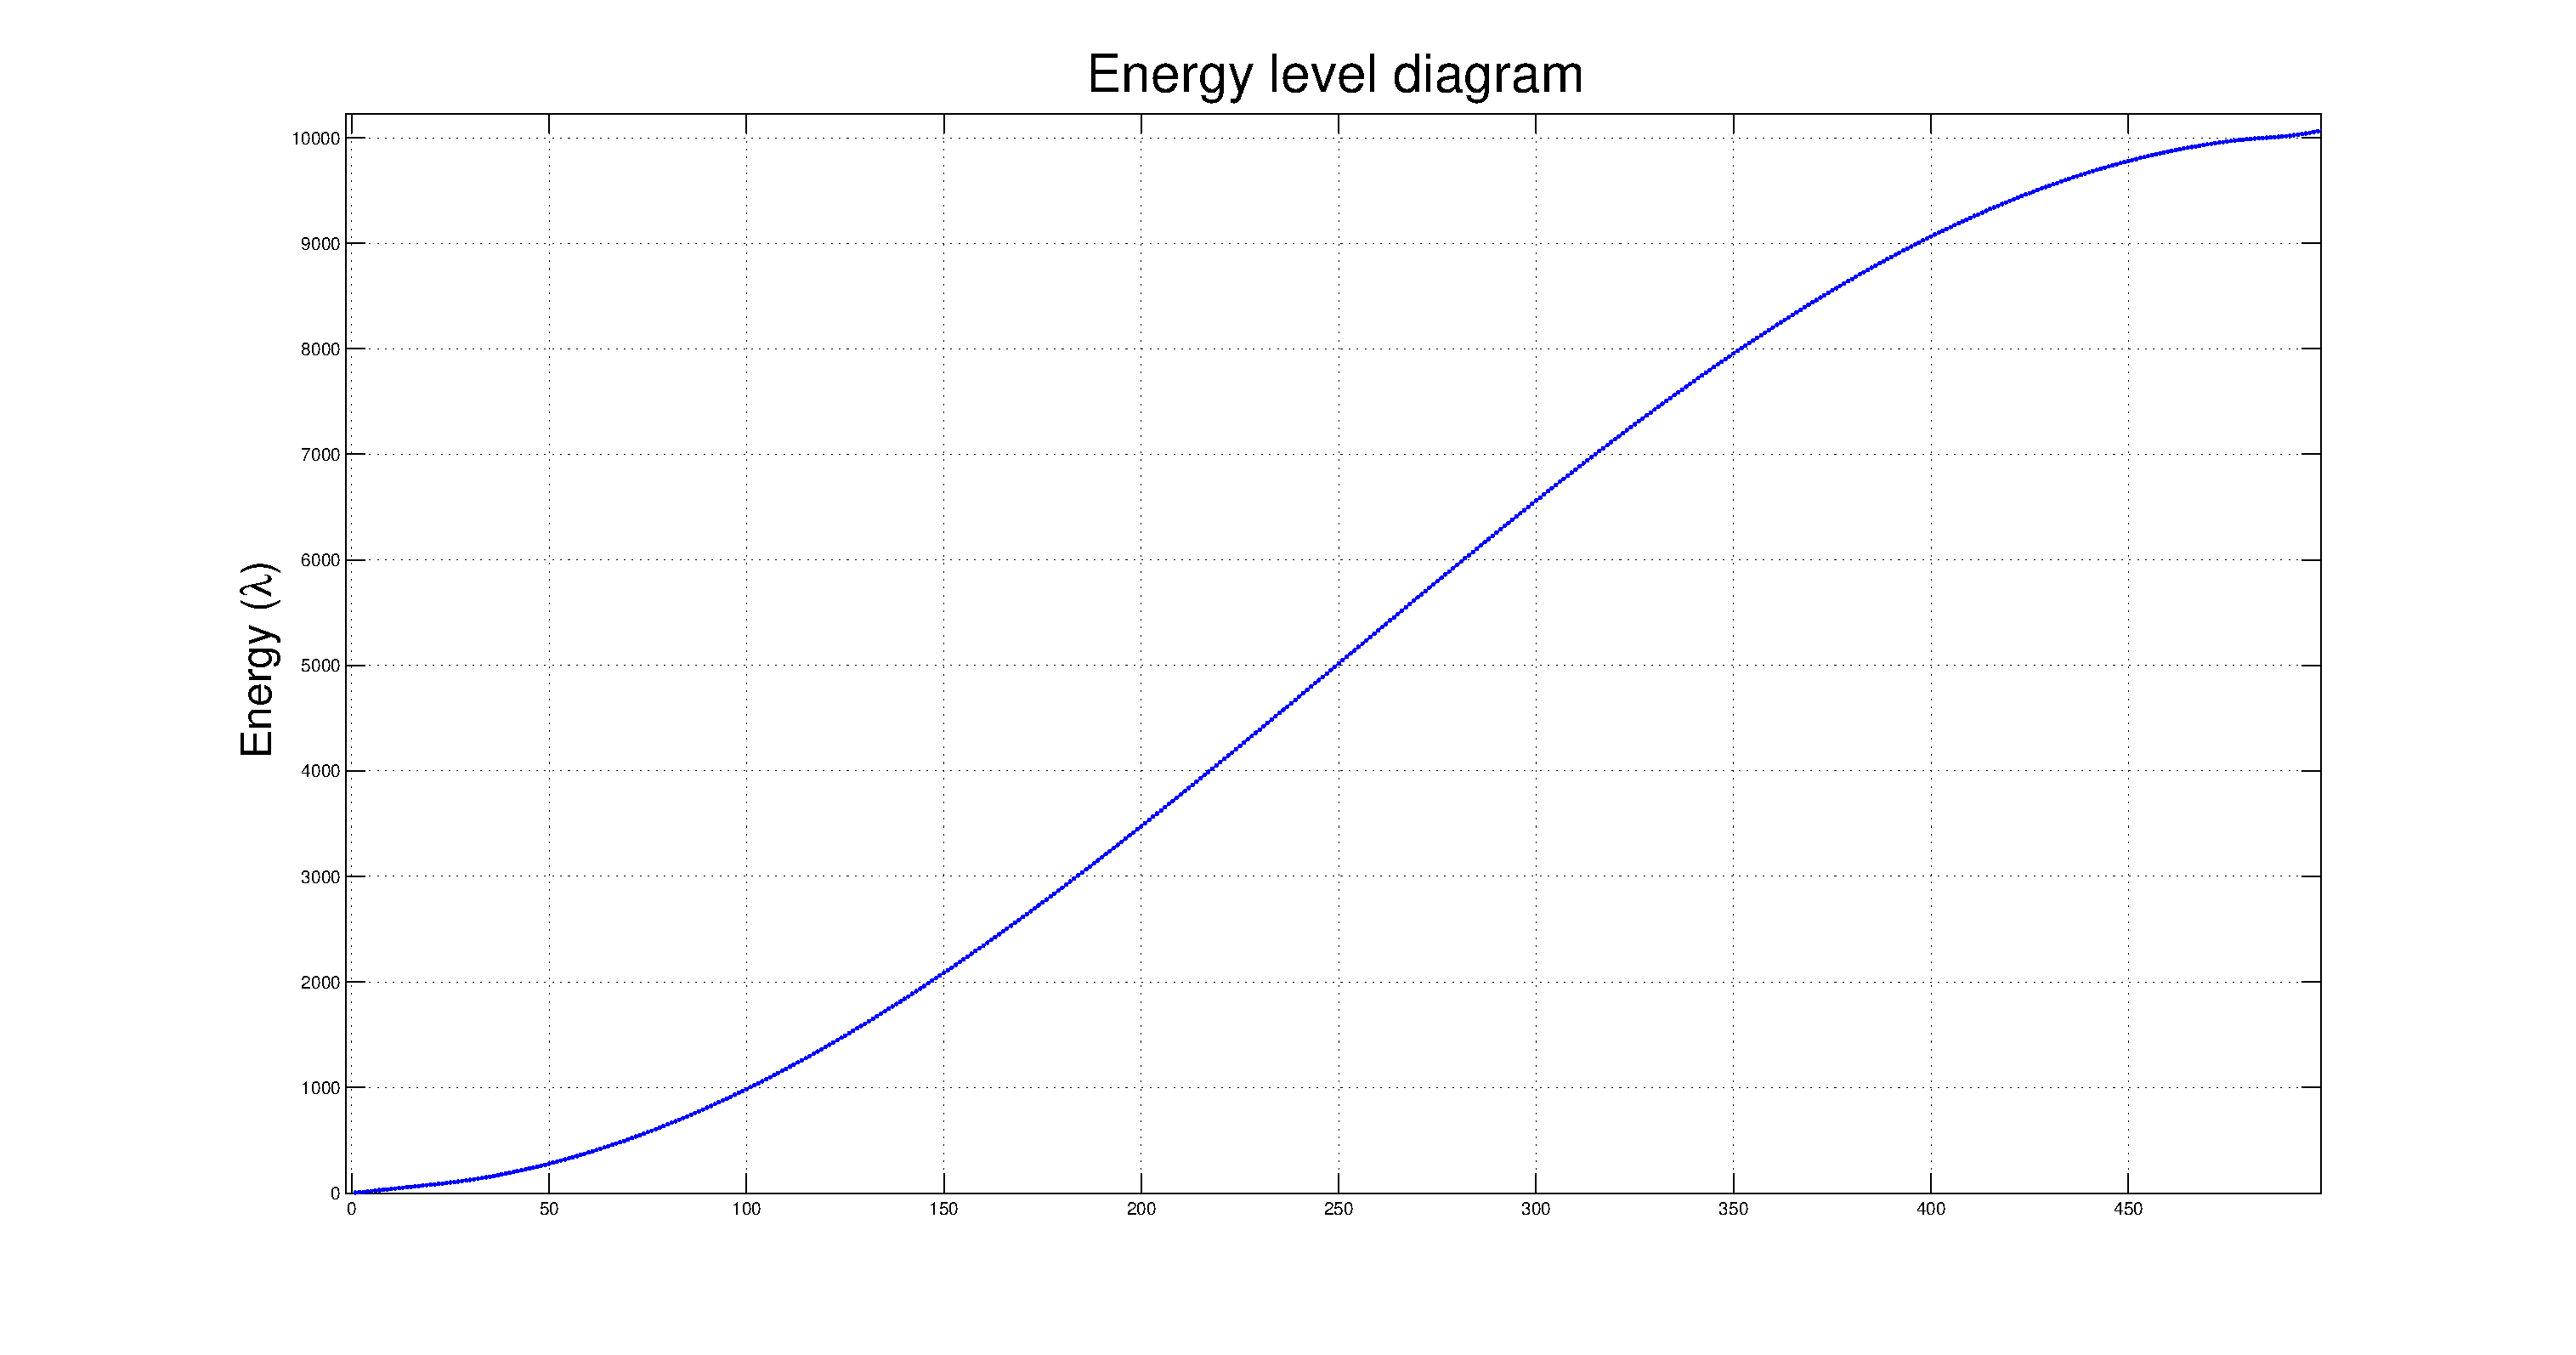
\includegraphics[width=16cm]{en}
	\caption{Energy levels in energy units $2m\alpha^2/\hbar^2$.}
	\label{fig:energy_levels_one_electron}
\end{figure}

Then, we calculated the radial solutions of our equation for the first four energy levels; they are shown in Figure \ref{fig:radial_solutions_one_electron}.

\begin{figure}[H]
	\centering
	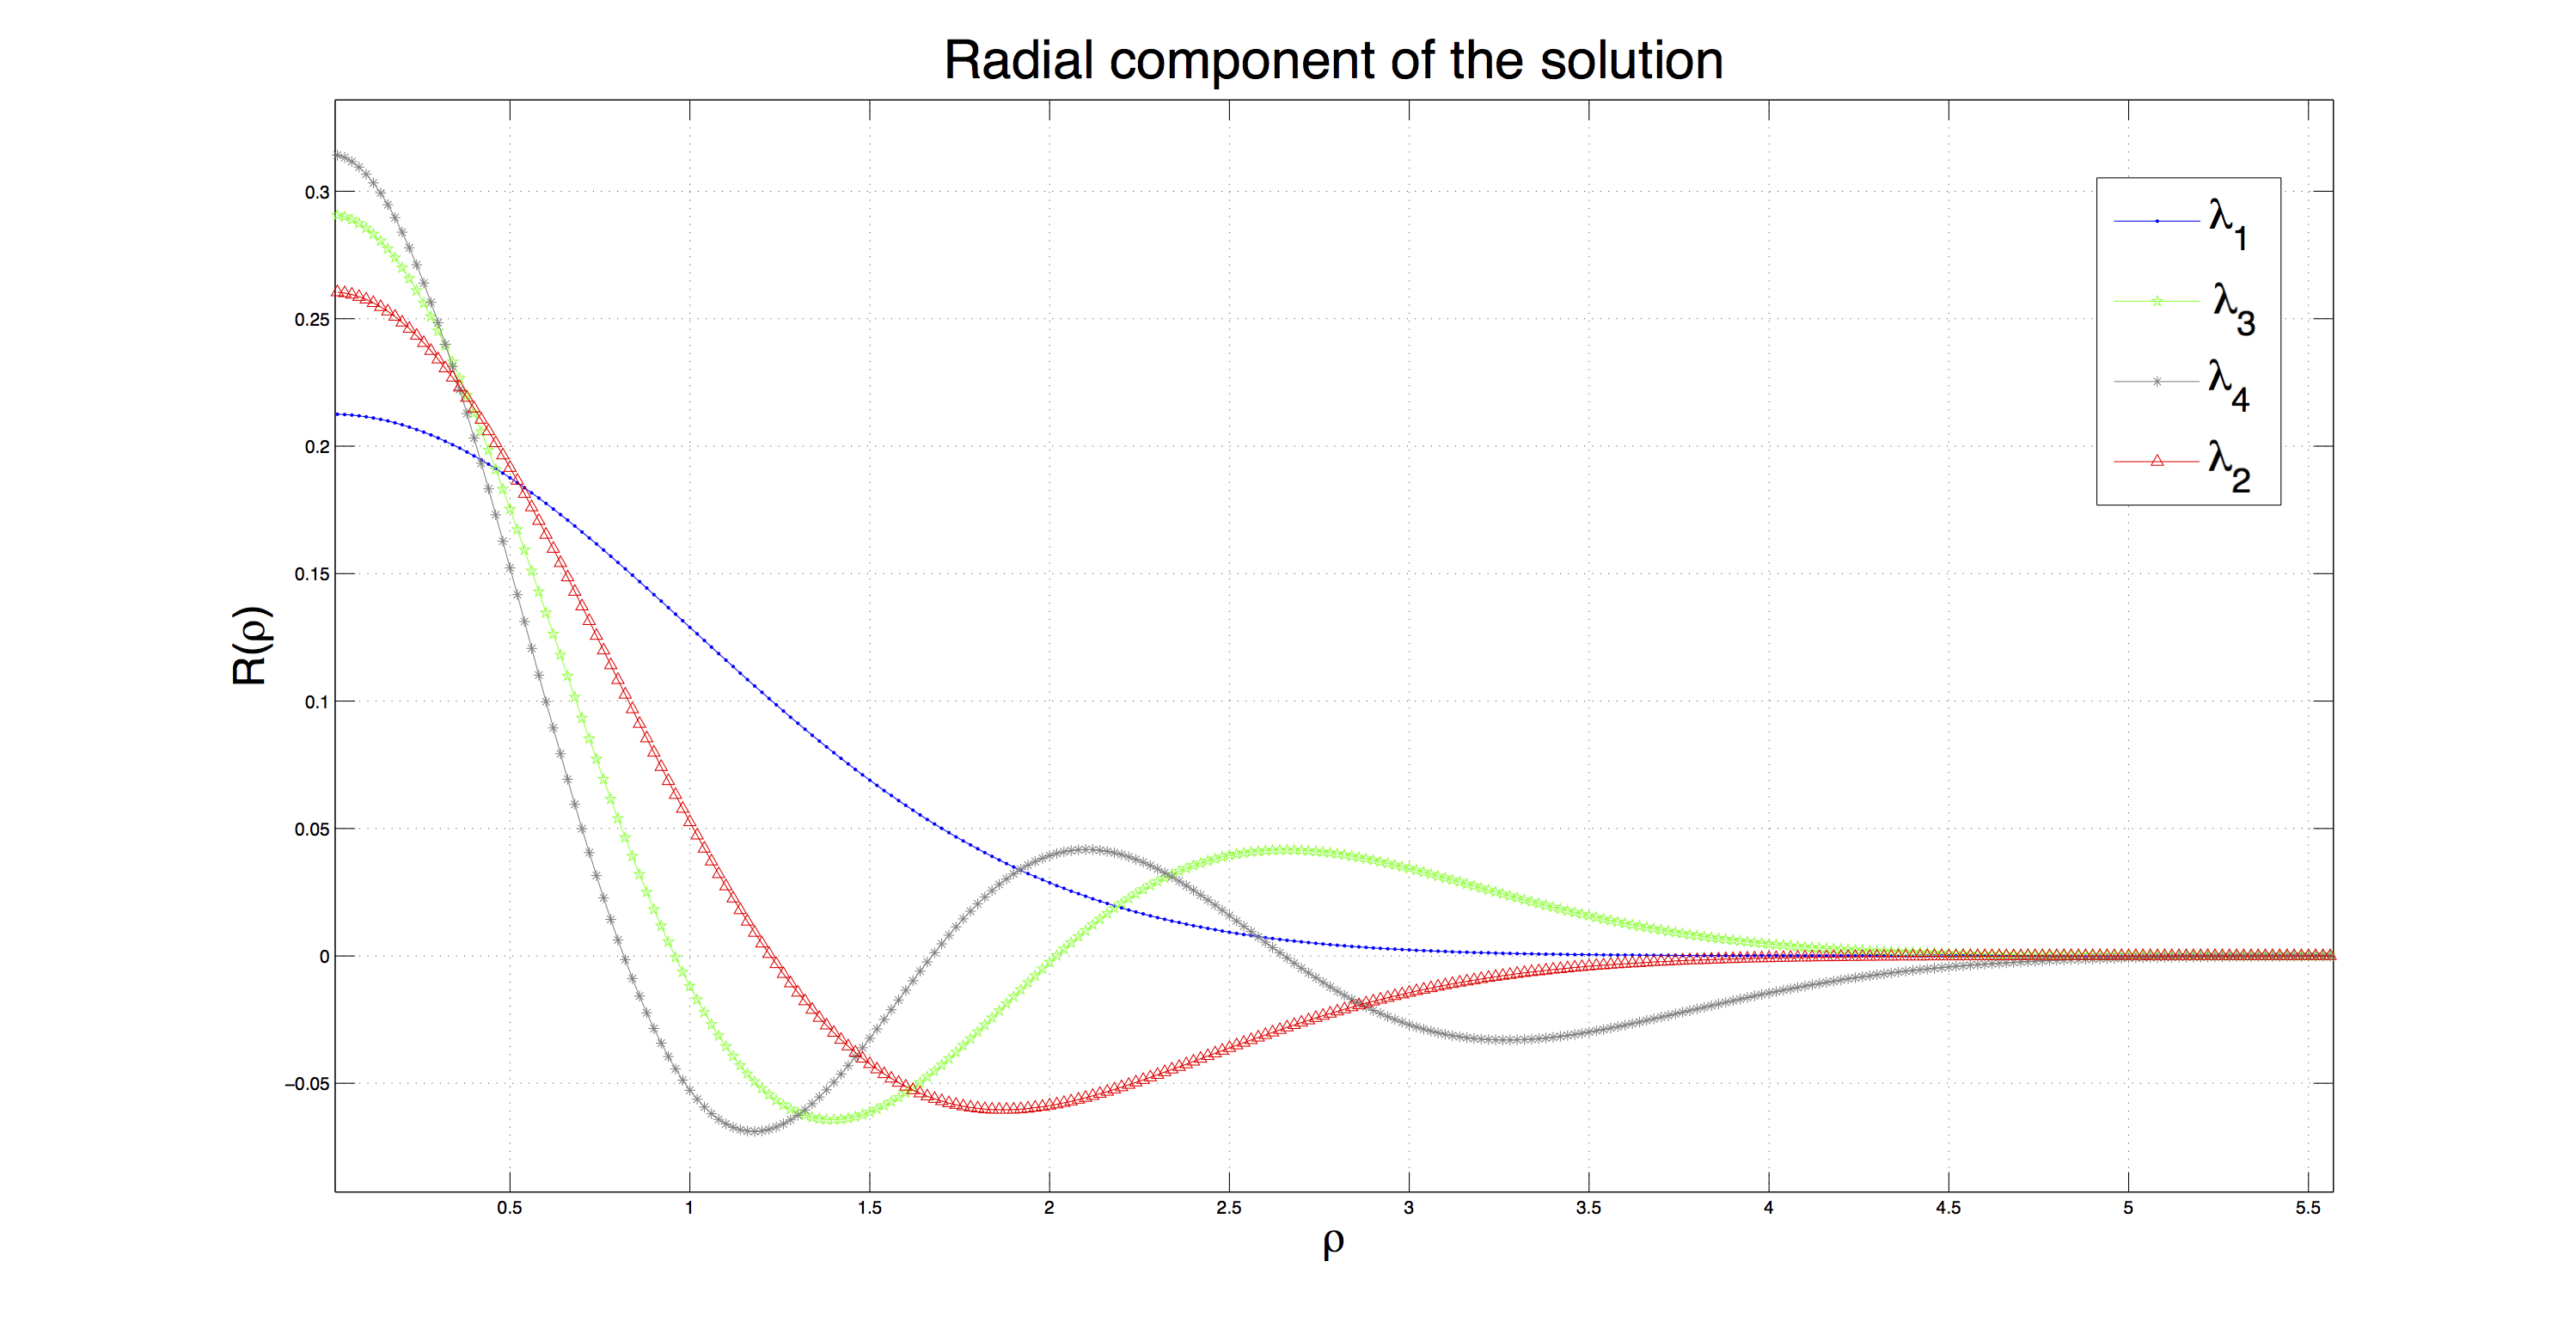
\includegraphics[width=16cm]{bla}
	\caption{Radial wave functions, for n going from 0 to 3.}
	\label{fig:radial_solutions_one_electron}
\end{figure}

As expected, the first solution has no nodes, while the second one has one node, the third one two nodes, and so on. However, the plot of the radial solution is not very significant; when we study particles, we are often more interested in predicting \emph{where} the particle is. Since the position can only be determined in a probabilistic way, we are precisely interested in the probability of finding the particle at a certain point for a given state (i.e., for a given energy value). By definition, this probability is the squared modulus of the wave function, integrated all over the space. Since the infinitesimal volume in spherical coordinates is $r^2\sin\vartheta\,dr d\vartheta d\phi$, we can exploit the symmetry properties of the solution and forget about all the angular components. That means that also the probability itself is symmetric at a given $r$, and so we can simply plot what we call a \emph{radial probability density} defined as $r^2R^2(r)$ to get an idea of how probability goes, no matter what angles $\vartheta$ and $\phi$ are. These probabilities densities are shown in Figure \ref{fig:probability_densities_one_electron}. 


\begin{figure}[H]
	\centering
	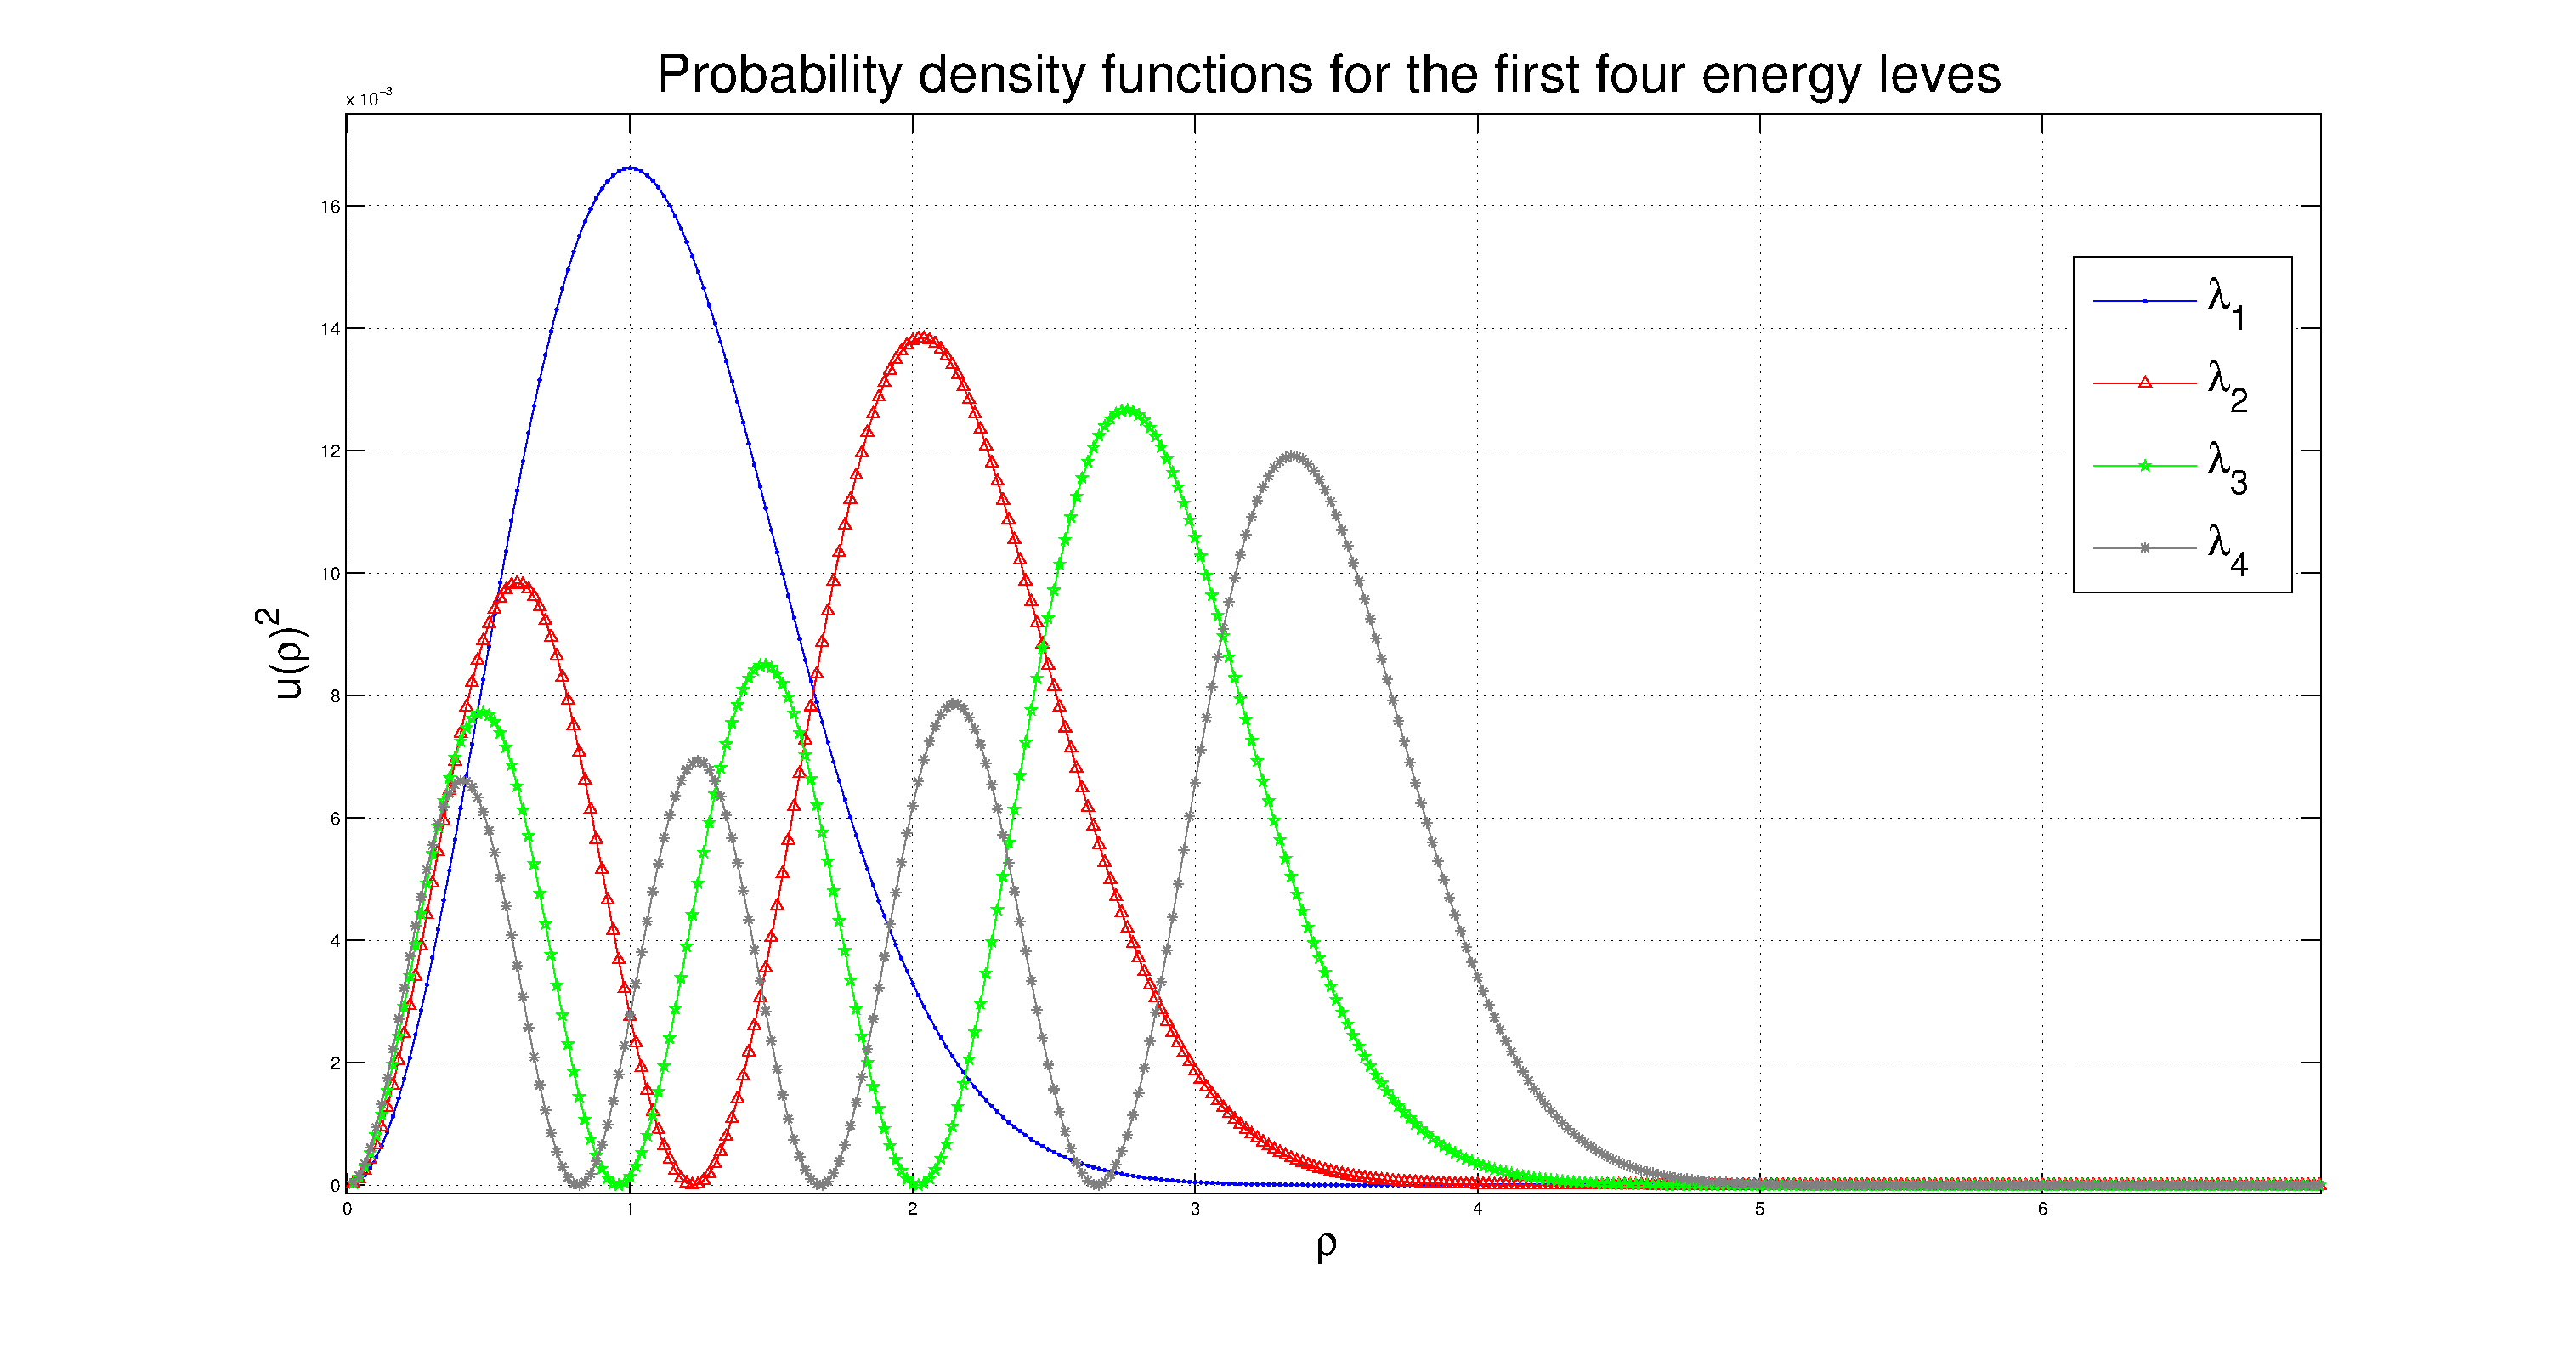
\includegraphics[width=16cm]{funct}
	\caption{Probabilty density functions for n going from 0 to 3, corresponding respectively to the lowest and the highest $\lambda$}
	\label{fig:probability_densities_one_electron}
\end{figure}

As it can be seen, for the first eigenvalue we have an high probability to find the electron near the atom, at a certain radius; increasing the quantum number $n$ we have the highest probability in finding the electron at a bigger and bigger radius, that is what we expected. It's interesting noting, however, that for $n>0$ we have also a lower probability in finding it at a distance that is smaller than the most probable radius with $n=0$, and for increasing values of $n$ this distance decreases. So, at major energies we most probably find the electron at major distances from the atom, but we also could find it near the atom.

These probability densities are pretty important when we study atoms; for example in our case we can define a $s$ \emph{orbital}, that is a sphere containing $90\%$ of the probability of finding the electron for a certain energy. For $\lambda_1$, we have what is called a $1s$ orbital, for $\lambda_2$ what is called a $2s$ orbital, and so on. Just as an example, the first three $s$-orbitals would look like those in Figure \ref{fig:s_orbitals}, where a darker color means a crest and the with color means a trough.

\begin{figure}[H]
	\centering
	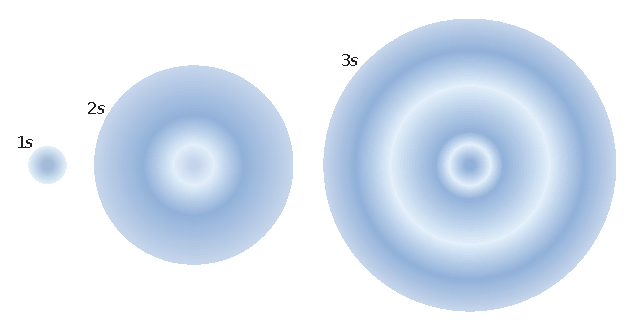
\includegraphics[width=10cm]{orbitals}
	\caption{$s$-orbitals (From \cite{oxtoby})}
	\label{fig:s_orbitals}
\end{figure}


\section{Two electrons in an harmonic potential with Coulomb repulsion}

We will now consider the case of two electrons subject to a harmonic potential and a repulsive interaction between the electrons. Lets first consider equation (\ref{chc}) where $\omega_r$ was set to 0.05. In this case the energy level diagram (figure(\ref{21})) is similar to the one that can be observed for the single electron. In this case the maximum value of $\rho$ chosen was of 80. In fact, as can be observed in figure (\ref{22}), the solution cannot be considered zero up until values of $\rho$ around 60. Choosing a lower value of $\rho_{max}$ would have lead to significant errors in the solution due to incorrect boundary conditions. 

\begin{figure}[H]
	\centering
	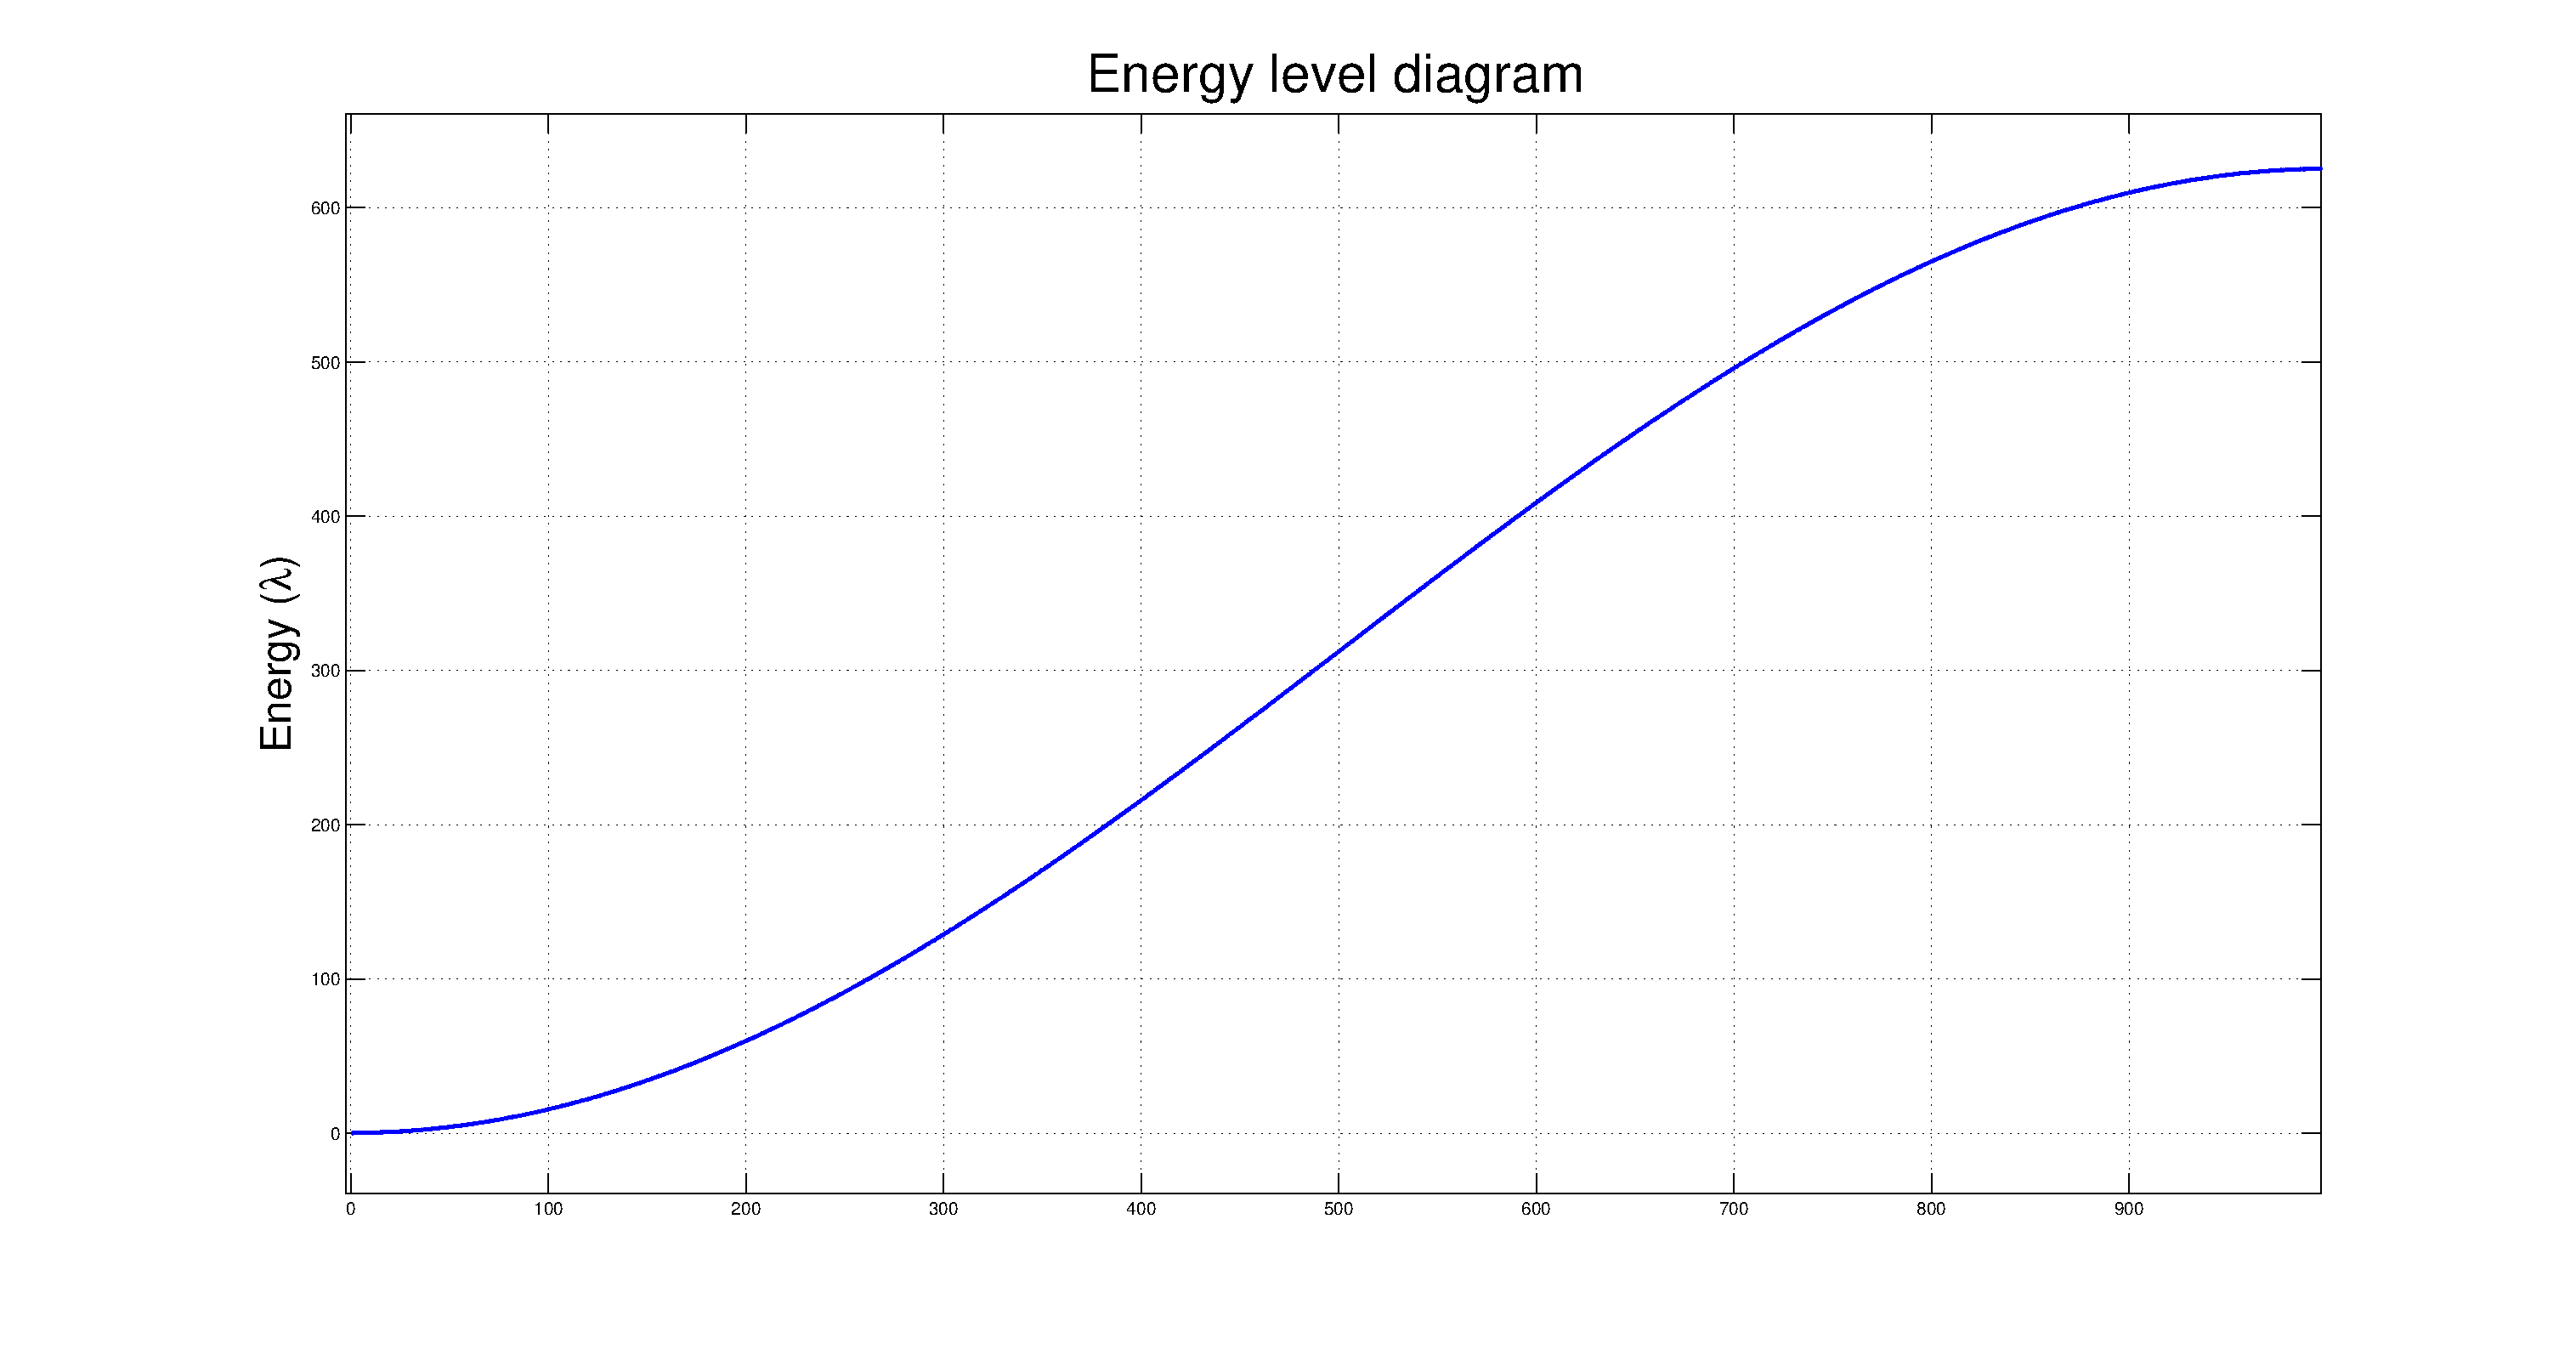
\includegraphics[width=16cm]{2elen}
	\caption{Energy level diagram for $\omega=0.05$ in energy units $2m\alpha / \hbar^2$}
	\label{21}
\end{figure}

\begin{figure}[H]
	\centering
	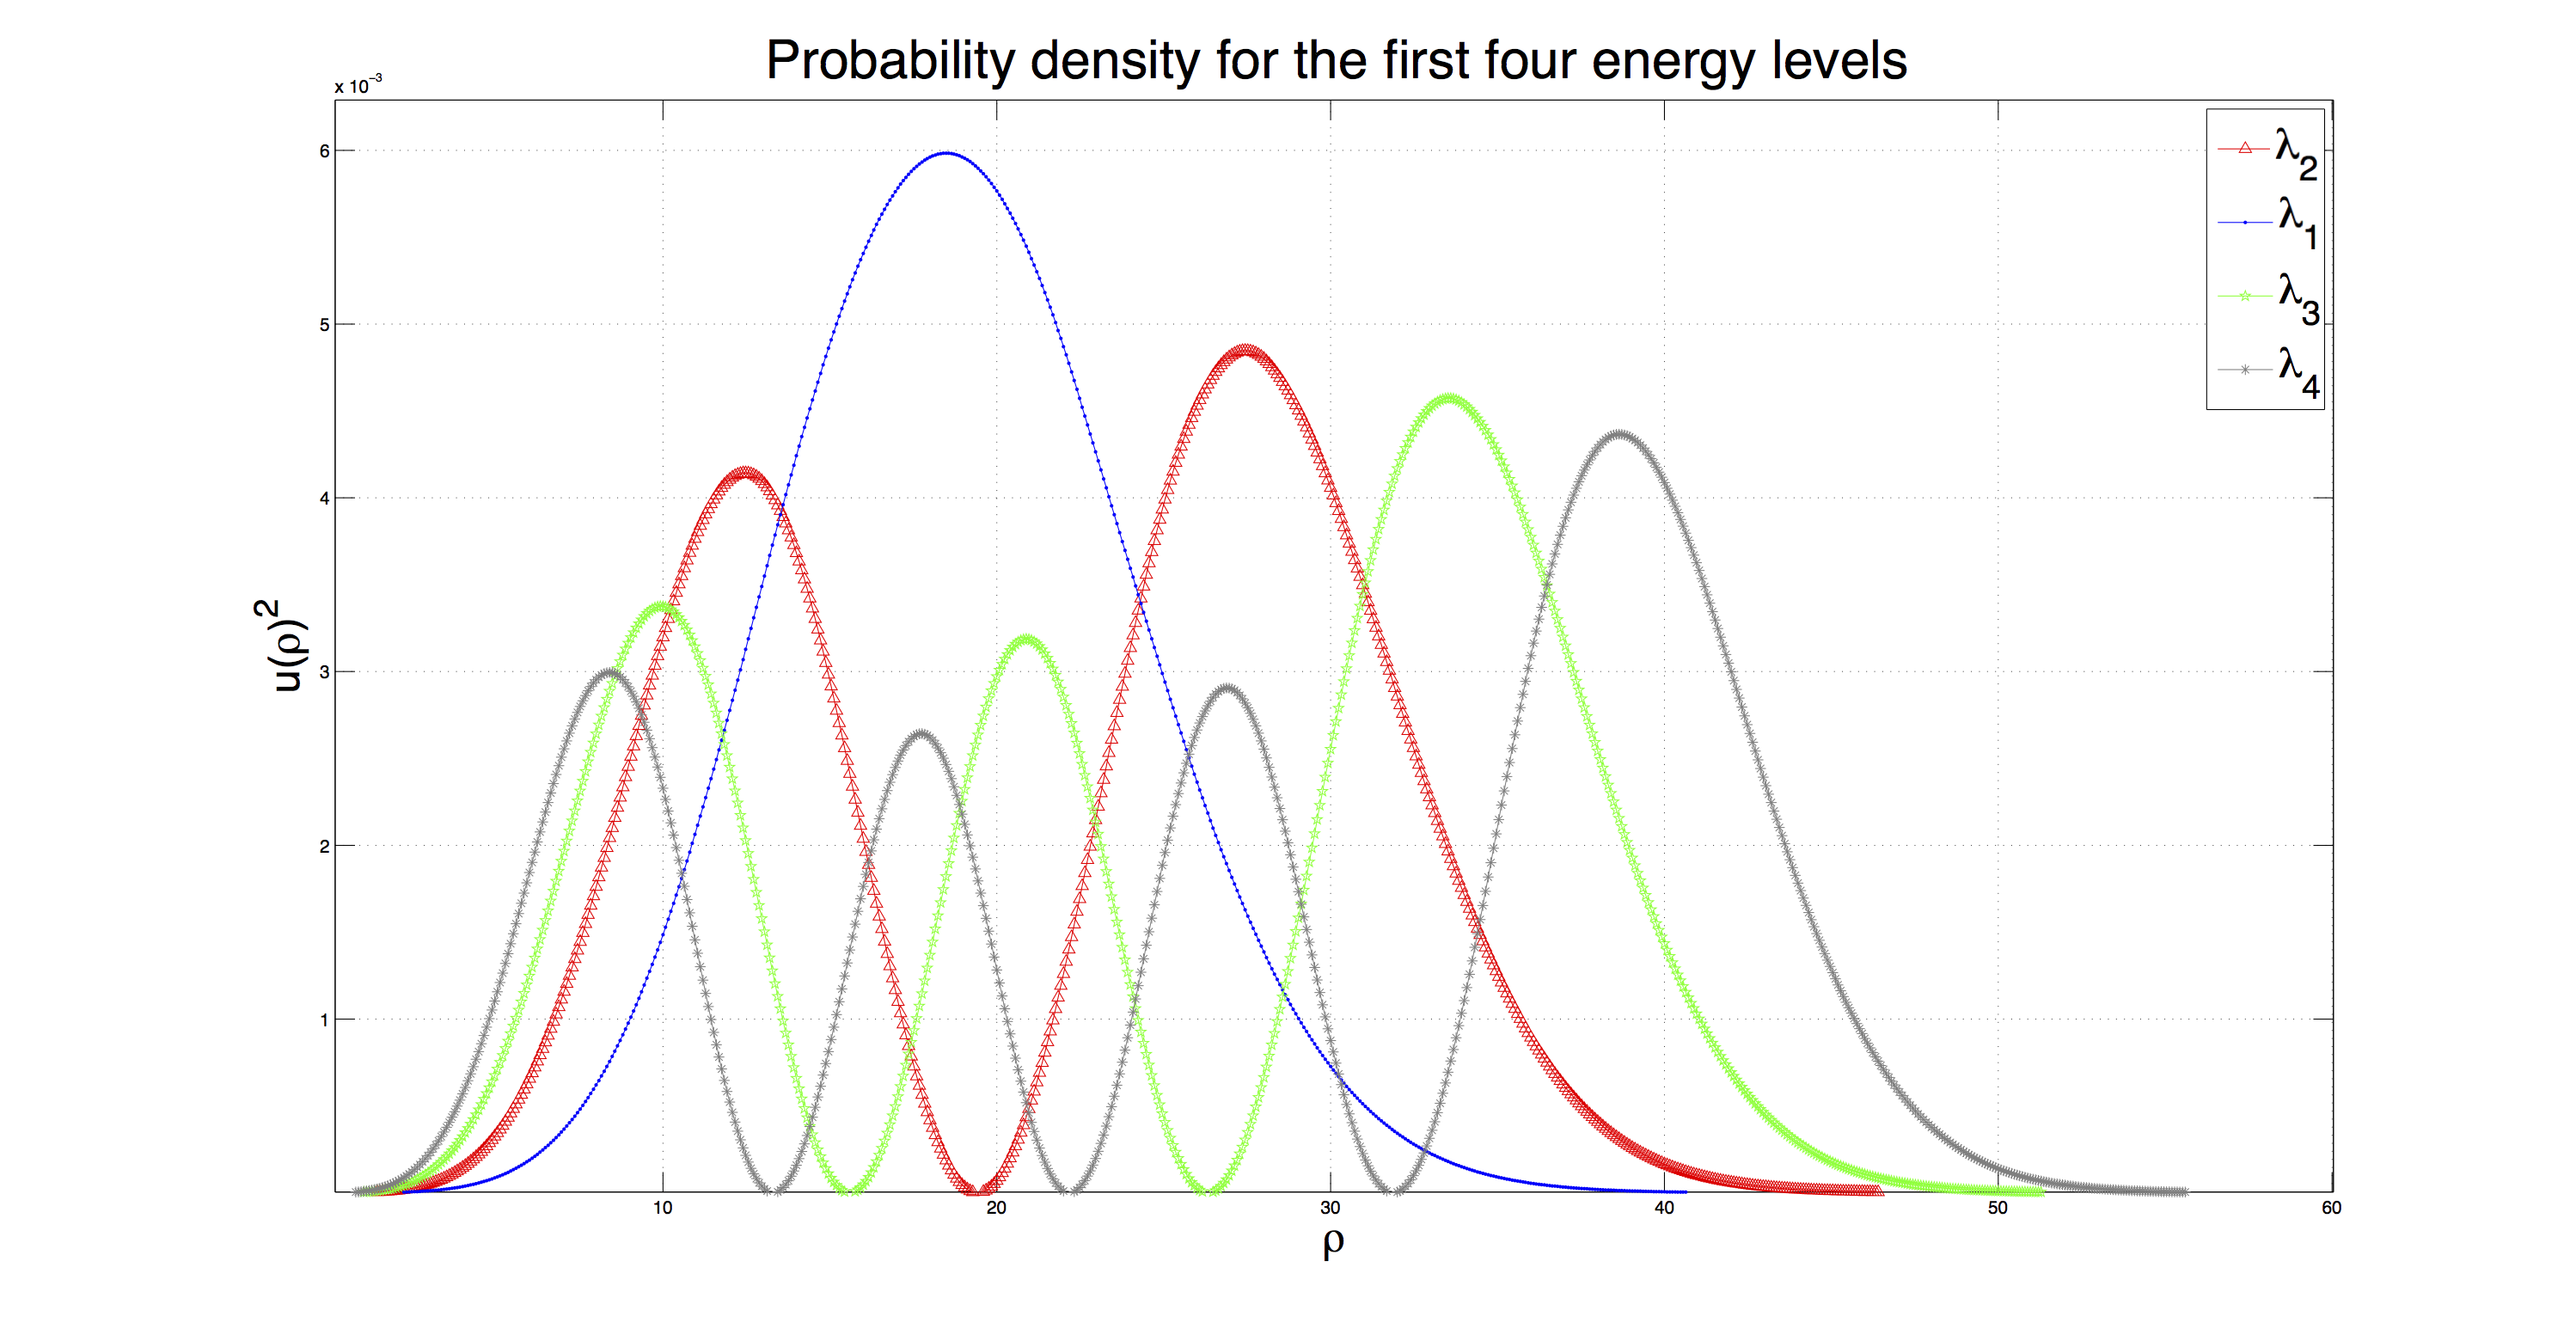
\includegraphics[width=16cm]{ciccione}
	\caption{Probability density function for n going from 0 to 3,  $\omega=0.05$. The number of crests determines the nalue of }
	\label{22}
\end{figure}

The result looks similar to the solution with 1 electron: for $n=0$ we have only one relative (and, in this case, absolute too) maximum, corresponding to the most probable radius, which in this case is the distance between the two electrons. Increasing n, the highest probabilities is found at increasing distances, but we also have a lower maximum at a radius that is smaller than the one for $n=0$. It is worth saying that, even if here the radius is the distance between the electrons, a smaller radius means, exactly as before, that the two negative particles are nearer to the atom.
\\

\begin{figure}[H]
	\centering
	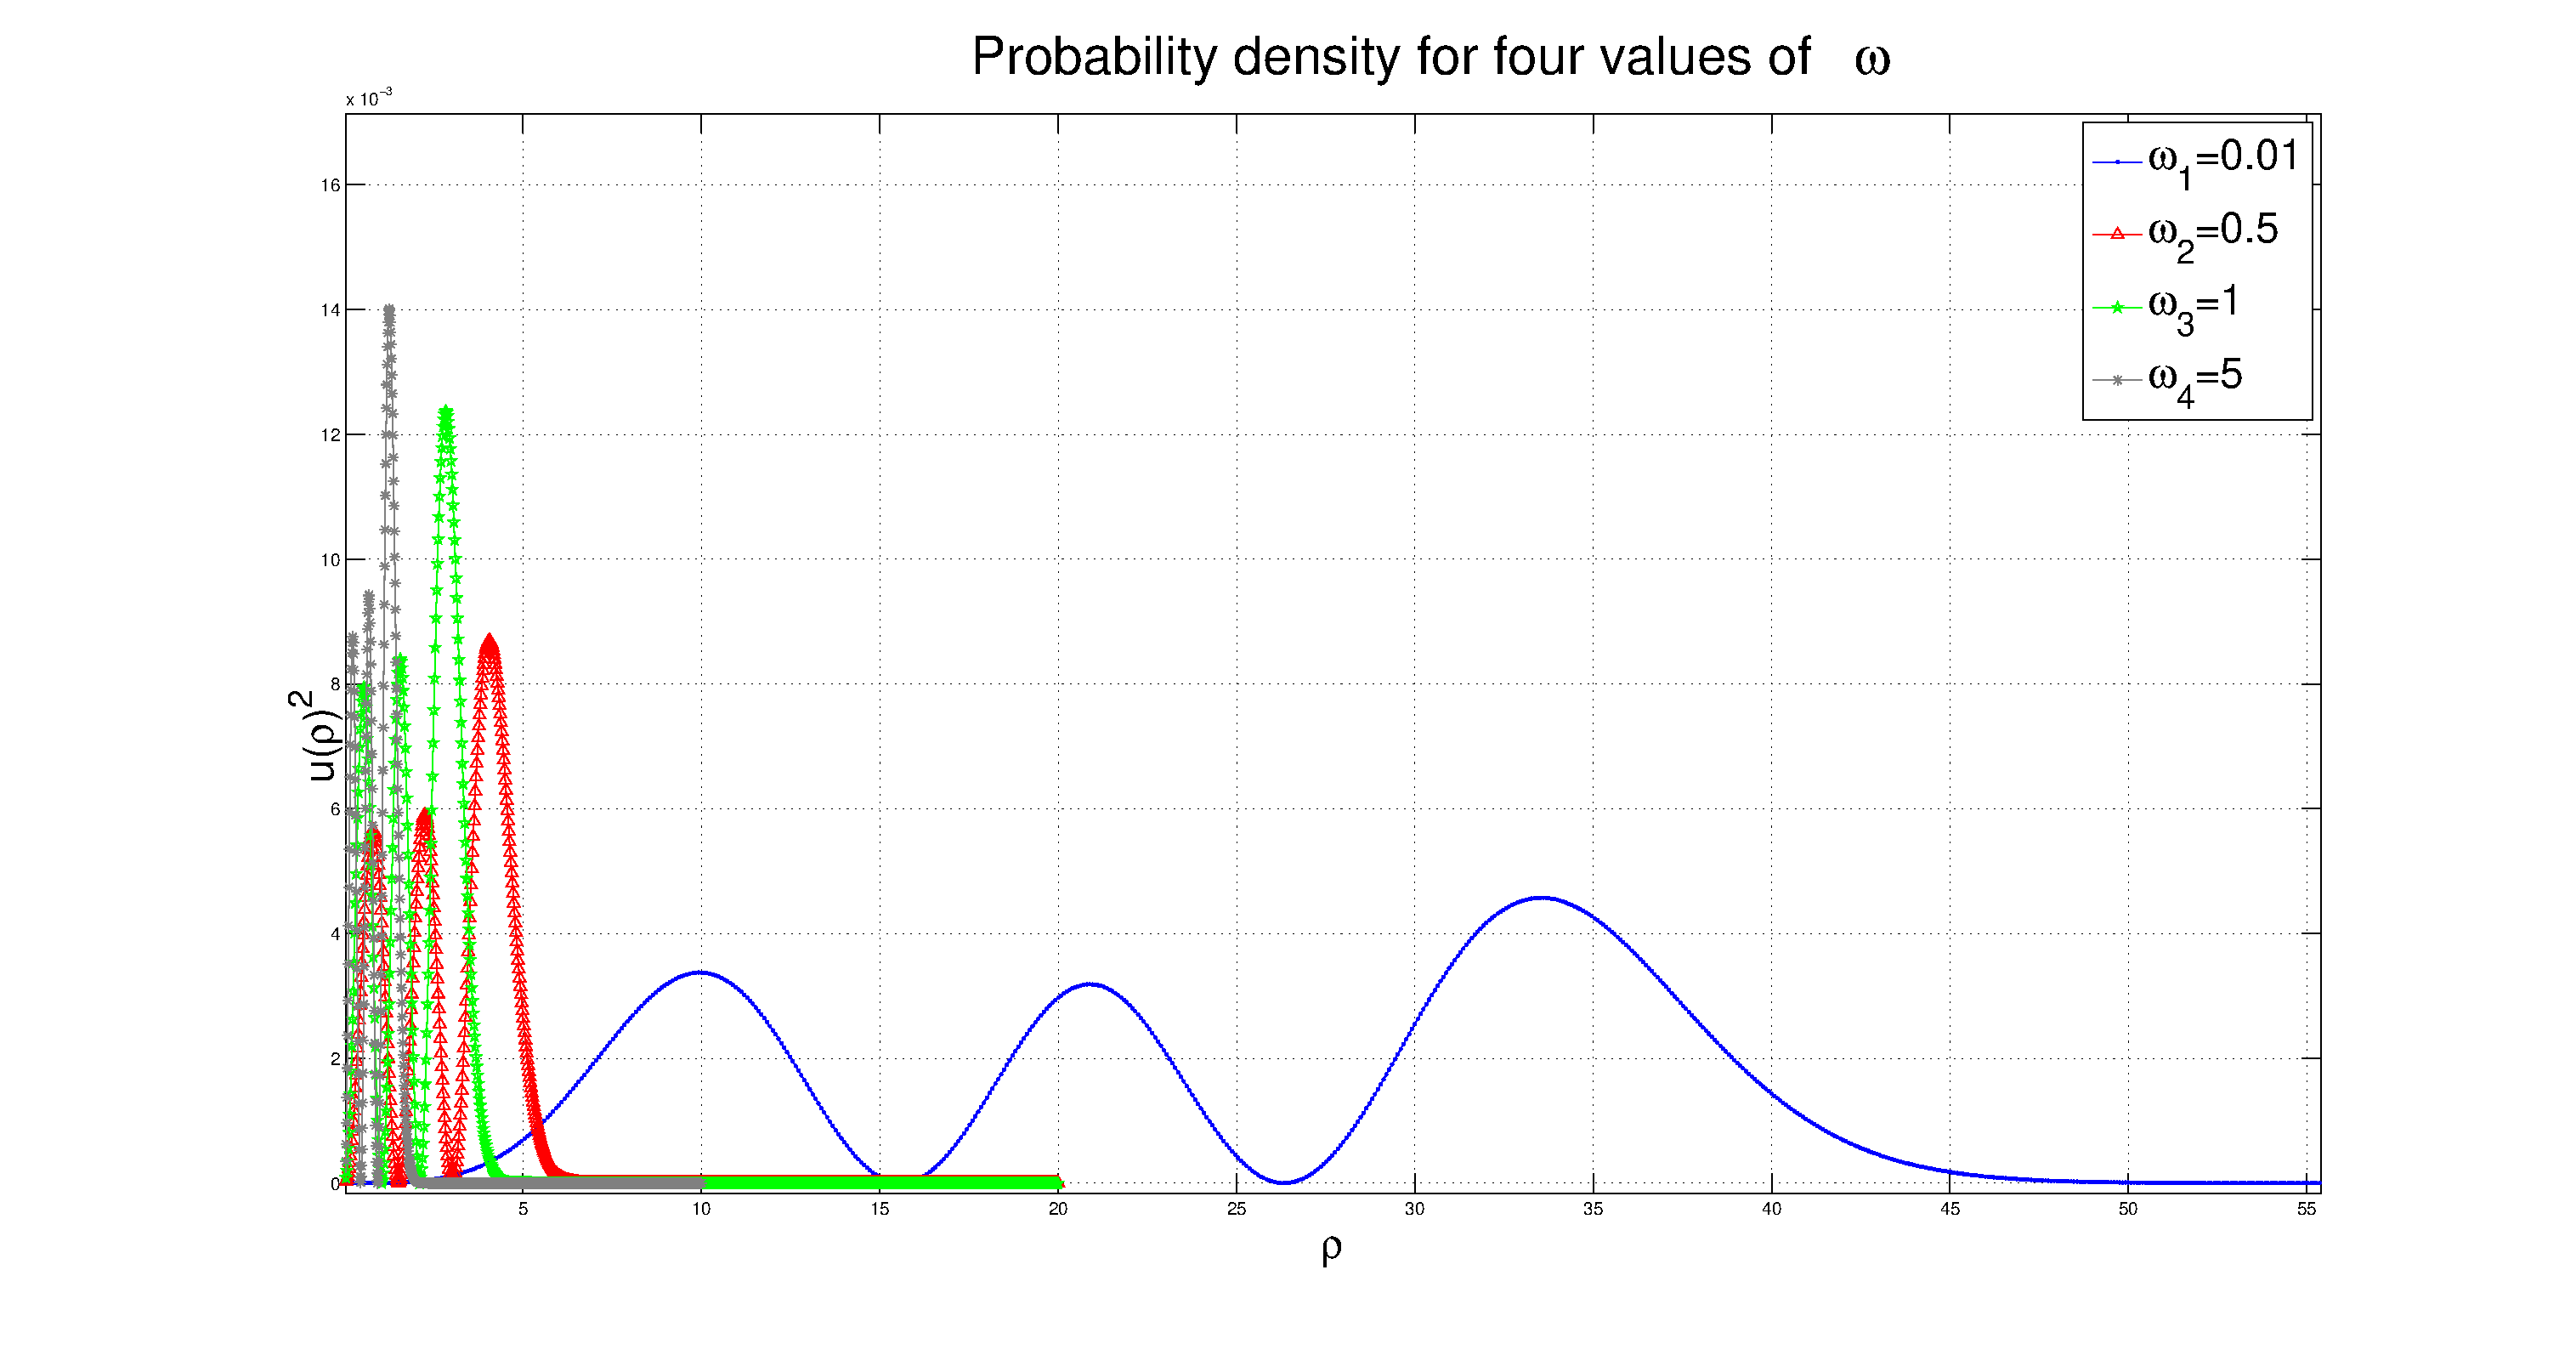
\includegraphics[width=16cm]{caccalog}
	\caption{$\lambda_3$}
	\label{25}
\end{figure}

To obtain a better view, we plot the graph on a logarithmic scale (even if in this way we lose the normalization of the density function):

\begin{figure}[H]
	\centering
	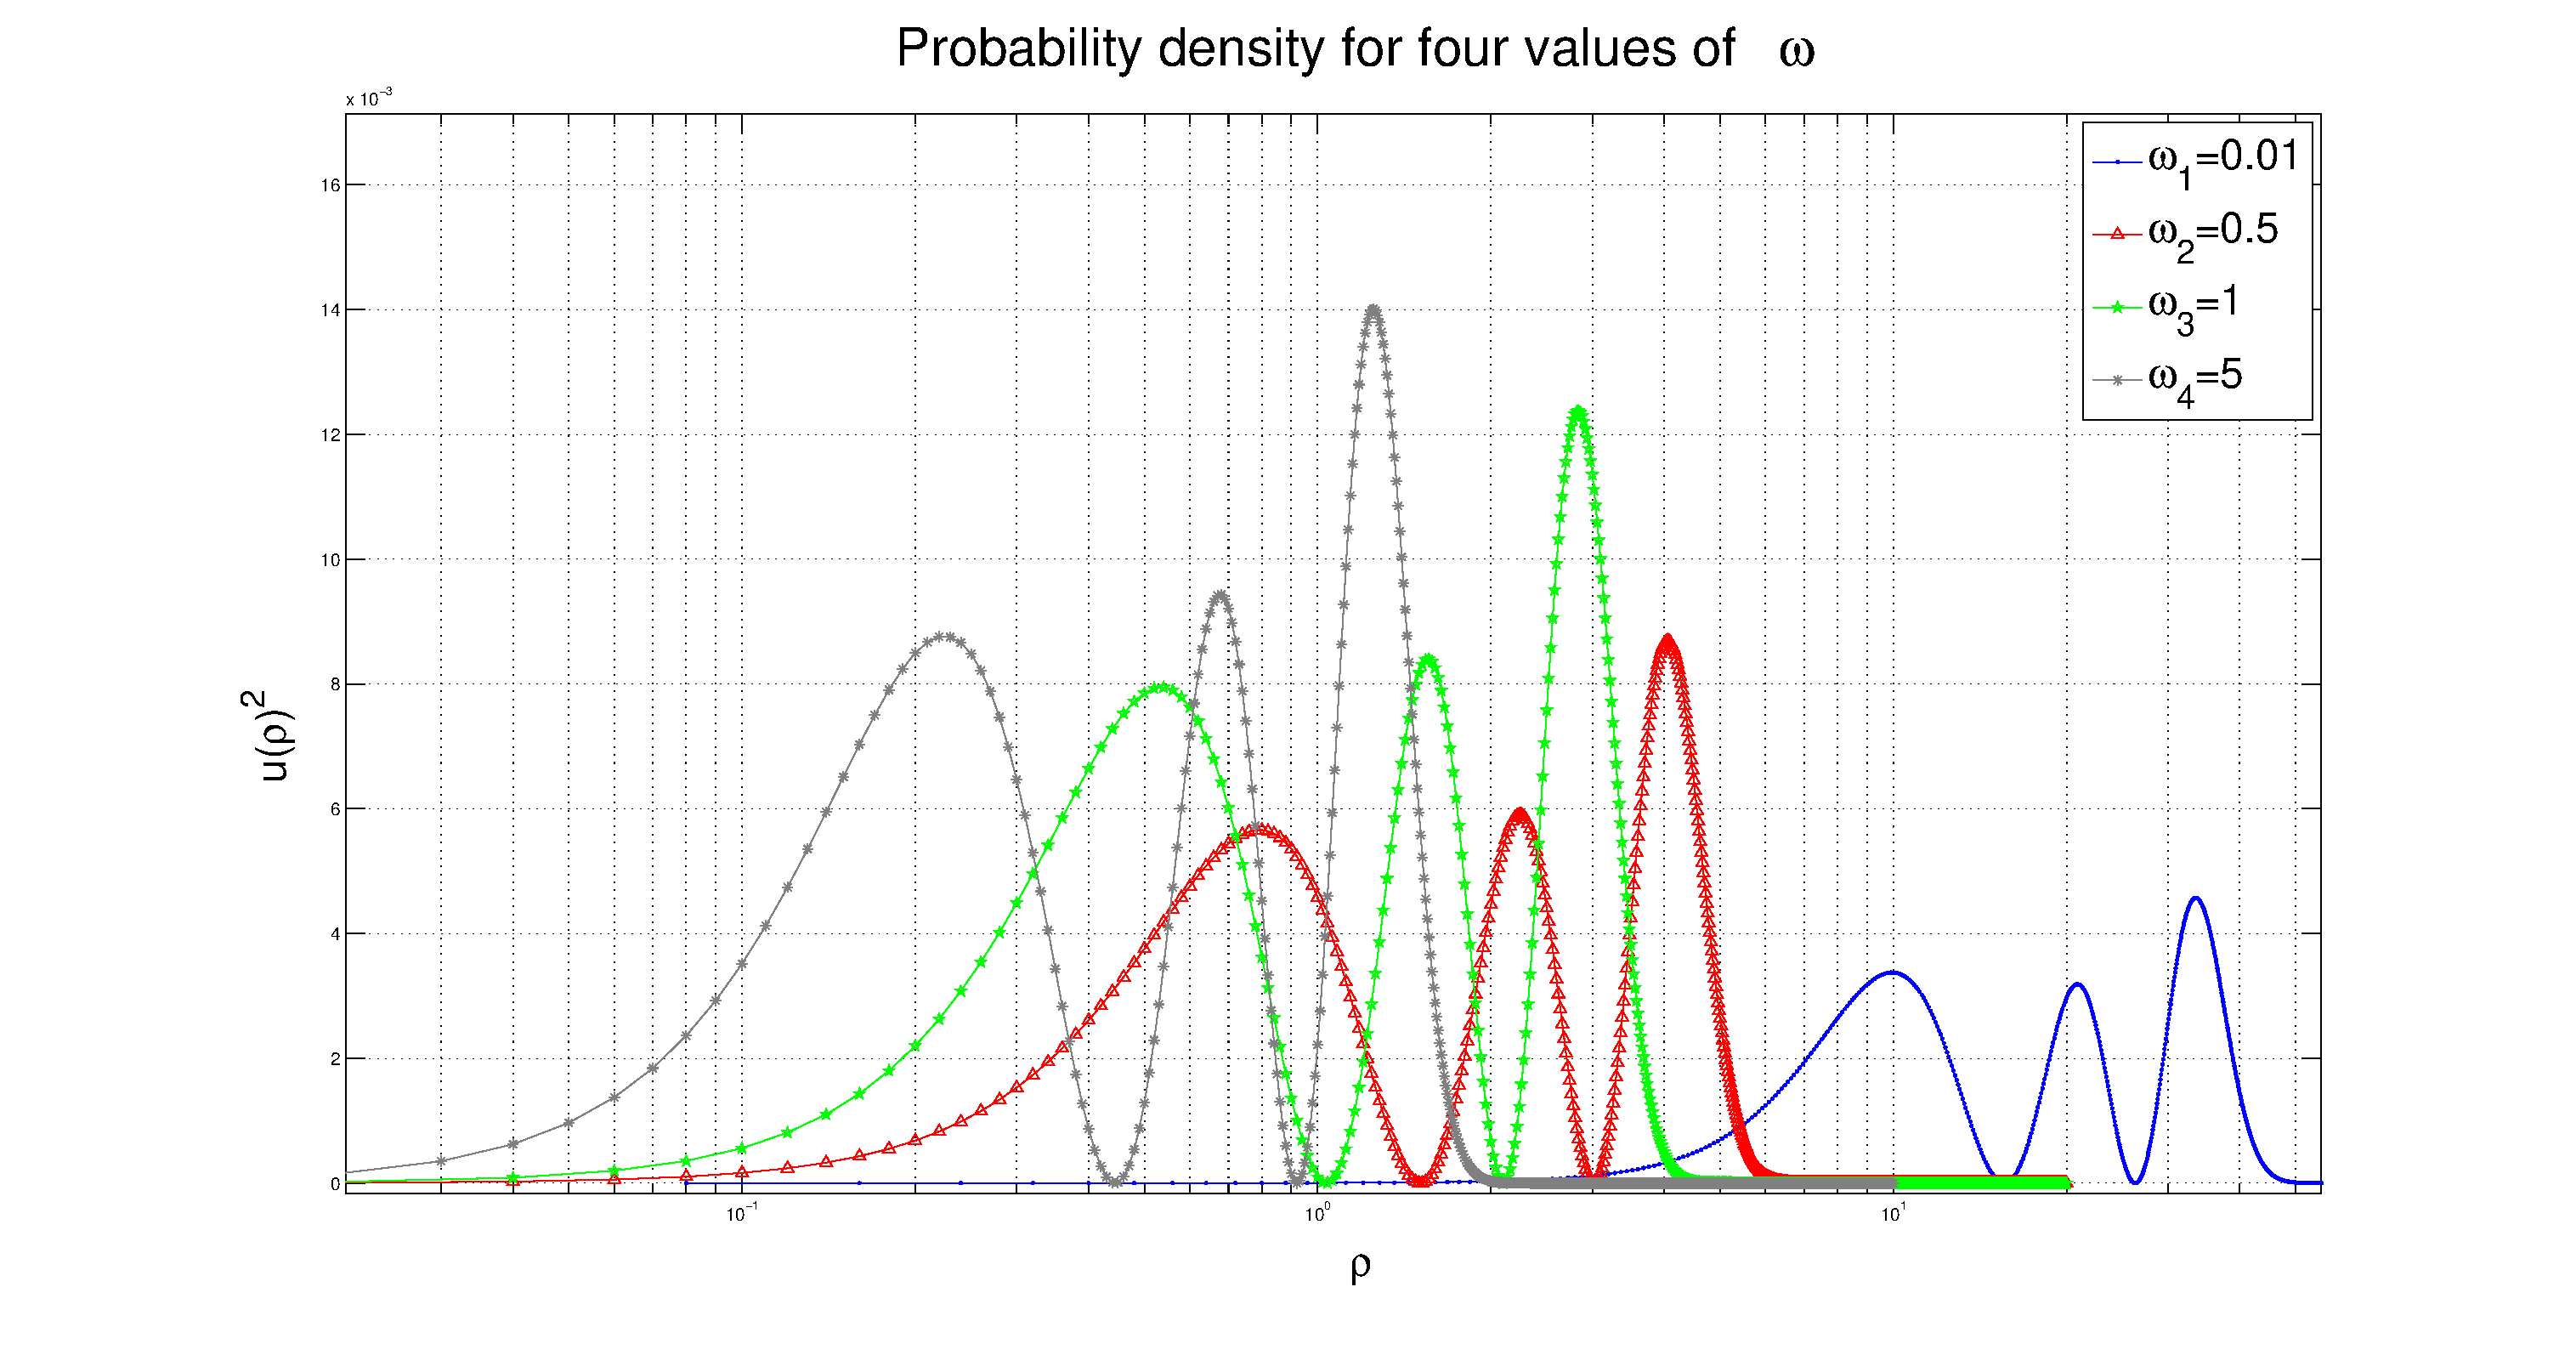
\includegraphics[width=16cm]{cacca}
	\caption{$\lambda_3$ - logarithmic scale}
	\label{23}
\end{figure}

For decreasing values of $\omega$, we notice that the two electrons tend to be at increasing distances from the atom: the probability density functions is translated to the left and spread on a larger range of $\rho$, which means that the maximums are lower. This is in accordance to the fact that a lower value of $\omega$ means a lower elastic constant, that is the electrons are less bonded to the atom.

\begin{figure}[H]
	\centering
	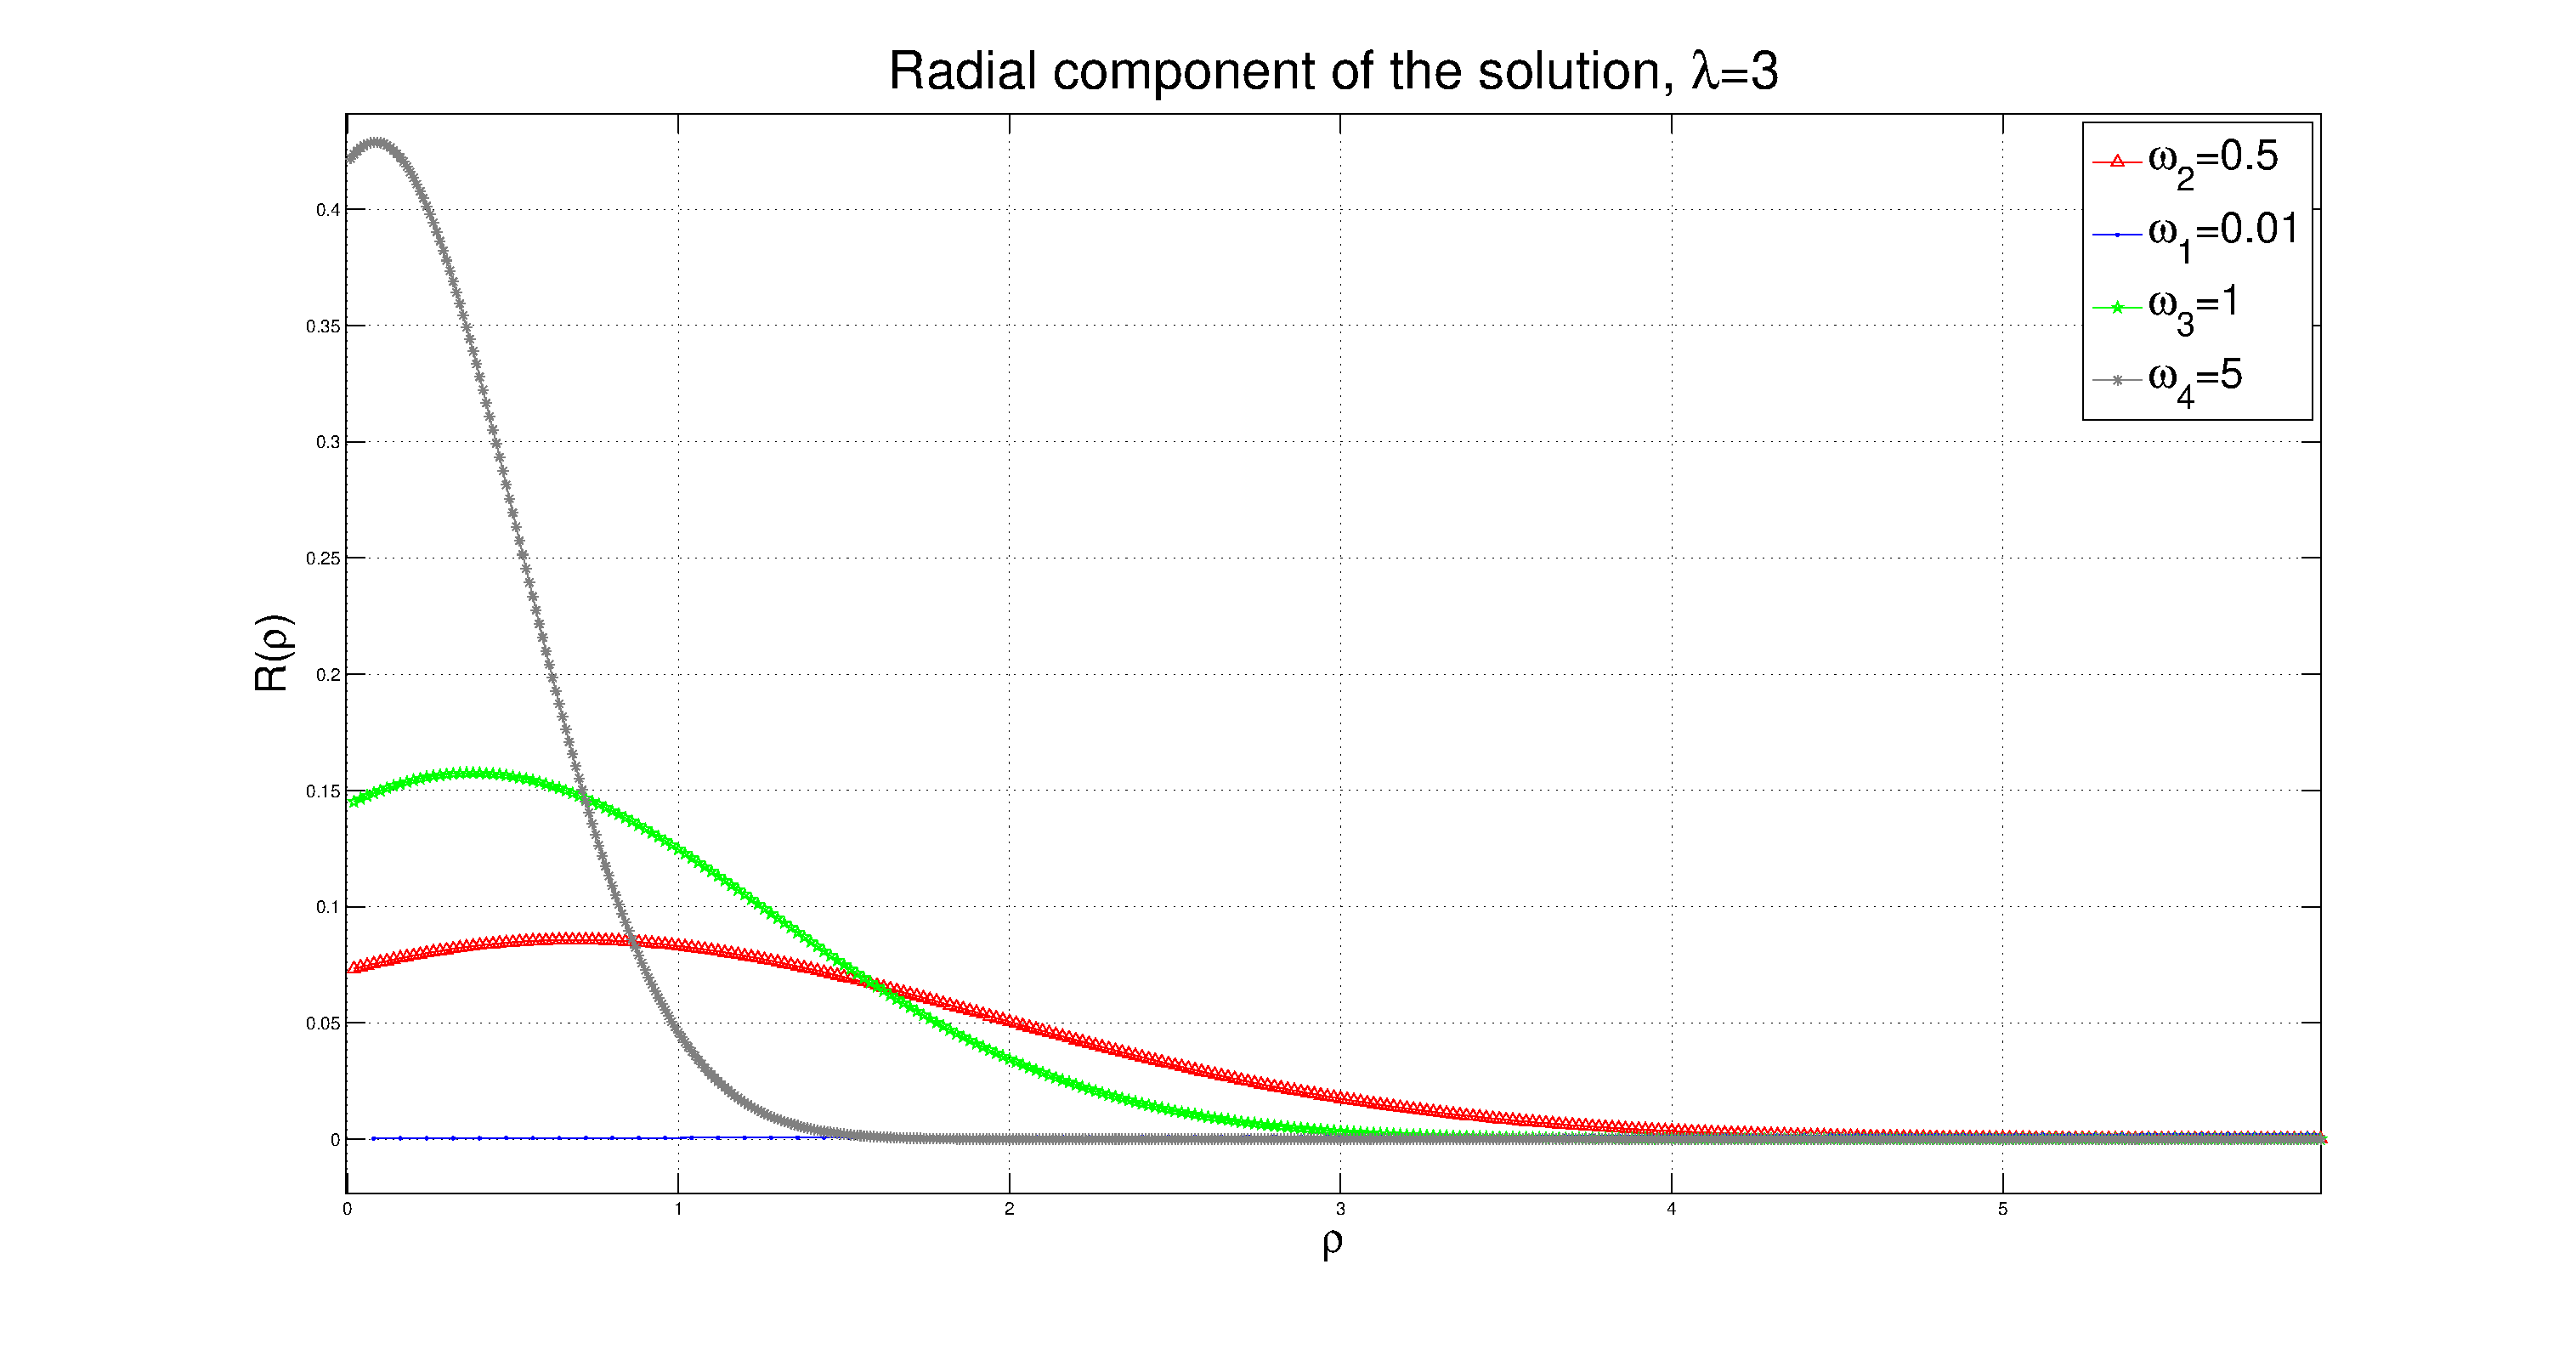
\includegraphics[width=16cm]{cacca2}
	\caption{$\lambda_3$}
	\label{24}
\end{figure}

\section{Conclusions and code}
We went to the conclusion that in order to solve Schr\"{o}dinger equation we need to find a compromise between the choice of the infinite point and the density in the solution points. These parameters vary based on the shape of the solution itself; so that for instance we had to adjust $\rho_{\max}$ to be equal to $80$ for the case $\omega_r = 0.01$, while the value $\rho_{\max}=10$ was enough $\omega_r = 5$.

We didn't manage to diagonalize matrices of dimension beyond $n=640$ because Jacobi's method is really slow: in fact the number of FLOPs go like $n^3$. For tridiagonal matrices, there are clever algorithms such as the one used in Armadillo or the well-known QR method.

All the code is stored at \url{https://github.com/matteosecli/Computational_Physics}. Since this is a private repo, you have to request access writing to \href{mailto:mattes@mail.uio.no}{mattes@mail.uio.no}.


\begin{thebibliography}{9}

\bibitem[Hjorth-Jensen]{morten}
  Morten Hjorth-Jensen,
  \emph{Computational Physics - Lecture Notes Fall 2014}.
  University of Oslo, 
  2014. 
%  \texttt{ISBN-13 978-0-321-85656-2}.

\bibitem[Press]{recipes}
  William H. Press, Saul A. Teukolsky, William T. Vetterling, Brian P. Flannery,
  \emph{Numerical Recipes}.
  Cambridge University Press,
  3rd edition,
  2007.
  \texttt{ISBN-13 978-0-511-33555-6}.
  
\bibitem[Oxtoby]{oxtoby}
  David W. Oxtoby, H.P. Gillis, Alan Campion,
  \emph{Principles of Modern Chemistry}.
  Brooks/Cole,
  7th edition,
  2012.
  \texttt{ISBN-13 978-0-8400-4931-5}.

\end{thebibliography}



\end{document}